\documentclass[french,12pt]{article}
\usepackage[utf8]{inputenc}
\usepackage[T1]{fontenc}
\usepackage{lmodern}
\usepackage[a4paper]{geometry}
\usepackage{babel}
\usepackage{xcolor}   
\usepackage{amsmath}
\usepackage{booktabs}
\usepackage{amsfonts}
\usepackage{amssymb}
\author{Thomas \bsc{Lantz}}
\usepackage{graphicx}
\usepackage{listings}
\usepackage{color}
\usepackage{float}
\restylefloat{table}
\usepackage{textcomp}
\usepackage{pgfplots,pgfplotstable}
\usepackage{url}
\usepackage{tikz}
\usetikzlibrary{arrows,backgrounds,mindmap,positioning,shadows,shapes}
\definecolor{listinggray}{gray}{0.9}
\definecolor{lbcolor}{rgb}{0.9,0.9,0.9}

\pgfplotstableset{
every head row/.style={before row=\toprule,after row=\midrule},
every last row/.style={after row=\bottomrule}}


\lstset{
	backgroundcolor=\color{lbcolor},
	tabsize=4,
	rulecolor=,
	language=C++,
        basicstyle=\scriptsize,
        upquote=true,
        aboveskip={0.5\baselineskip},
        columns=fixed,
        showstringspaces=false,
        extendedchars=true,
        breaklines=true,
        prebreak = \raisebox{0ex}[0ex][0ex]{\ensuremath{\hookleftarrow}},
        frame=single,
        showtabs=false,
        showspaces=false,
        showstringspaces=false,
        identifierstyle=\ttfamily,
        keywordstyle=\color[rgb]{0,0,1},
        commentstyle=\it\tt\color[rgb]{0.133,0.545,0.133},
        stringstyle=\color[rgb]{0.627,0.126,0.941},
        inputencoding=utf8
        }

\lstset{escapeinside={(*@}{@*)}}
\lstset{includerangemarker=false,rangeprefix=\/\/\#\ ,% curly left brace plus space
  rangesuffix=\ \#}% space plus curly right brace



\begin{document}
\begin{titlepage}
\begin{center}
  \Huge
  \textbf{UFR de Mathématiques et d'Informatique de Strasbourg}
  \par \vspace{2 cm}
  \textbf{Rapport de Stage}
  \par \vspace{1 cm}
  \emph{Wrapping Python}
  \par \vspace{5 cm}
  \bsc{Lantz} Thomas
  \par \vspace{2 cm}
  \bsc{M1 CSMI}
  \par \vspace{3 cm}
  \normalsize{\today}\\
  \end{center}
\end{titlepage}

\newpage
\tableofcontents
\newpage

\section*{Remerciements}
Tout d'abord, je tiens à remercier M. Prud'homme pour m'avoir proposé ce sujet, ainsi qu'à M. Ancel, mon responsable de stage, pour m'avoir aidé et soutenu tout au long de ce stage, malgré les difficultés rencontrées. Je remercie également M. Huber ainsi que l'équipe informatique de l'UFR pour leurs aides sur tout ce qui concerne la gestion des comptes et problèmes informatiques. Enfin, je remercie également mes camarades de stages, Marion, Benjamin et Mamadou, pour leurs soutiens ainsi que la bonne ambiance qu'ils ont fait régner durant ces deux mois.

\newpage
\part{Rapport}
\section{Introduction et présentation des outils}

Afin de débuter ce rapport, commençons par énoncer le sujet sur lequel j'ai travaillé et présenter par la même occasion certains des différents outils qui seront utilisés au cours de celui-ci.

\subsection{Introduction au sujet}

La compilation d'un fichier en C++ est nécessaire à chaque modification de celui-ci et elle est d'autant plus longue que son contenu est grand, notamment de part la présence de nombreux headers dans le code, affectant alors le parser à la compilation, ou par le nombre de templates ou méta templates qui peuvent être présent dans le code, par exemple. Bien sûr la taille du programme joue également un rôle important dans ce temps de compilation.
\newline

Alors quand il est question de ne modifier qu'un paramètre, la dimension des éléments du maillage par exemple, pour divers tests, le fait de devoir recompiler à chaque changement va nous coûter pas mal de temps. Même si il est possible en pratique de modifier nombres de paramètres grâce à l'utilisation d'options que l'on appelle alors par ligne de commande à l'exécution, cela ne permet pas de résoudre ce problème dans tous les cas.
\newline

Le sujet de mon stage, le Wrapping Python du code Feel++, a pour but d'essayer de corriger cela. En effet, le wrapping consiste à récupérer des classes et méthodes déjà implémentées (ici en Feel++/C++) afin de pouvoir créer un module Python, c'est à dire une librairie contenant la définition de différents objets utilisable en Python, dans l'environnement C++ à partir d'une autre librairie partagée déjà existante qui liera ces deux langages. Ce module nous permettra de les utiliser dans un nouveau langage (ici Python) grâce à des outils divers que l'on présentera après.
\newline

Le Python étant un langage non compilé mais interprété,  la modification dans le script d'un paramètre n'entraînera pas de recompilation et l'exécution se fera de suite après cela. Ainsi il nous suffira donc de construire le module Python à partir des outils et codes déjà implémentés,  de compiler celui-ci une seule fois, on pourra alors utiliser toutes les méthodes et classes ainsi récupérées dans un script Python.
\newline

Après avoir présenté certains outils qui seront utilisés lors de ce stage, on pourra alors commencer la présentation du travail effectué lors de ces deux mois, en essayant de part ce fait vous expliquer le fonctionnement et l'utilisation du wrapping Python.

\subsection{Environnements de développement}

\subsubsection{Trello}

Trello est une plateforme d'organisation de travail en ligne. Elle est organisée sous forme de board (ou tableau) dont on définit l'accès aux différents participants.
\newline

Chaque board peut être décomposé en sous-sections que l'on créera et qui contiendra des cartes définissant les différentes tâches voulues.
Chaque carte, outre son titre, peut être complétée avec toutes sortes d'informations comme des liens, des images ou des paliers à accomplir pour la réalisation d'une tâche et peut être limitée à modification par les participants voulues.
\newline

De même, ces cartes peuvent à tout moment être déplacées entre les différentes sections du board, ce qui permet par exemple de voir dans notre cas le travail à faire, celui qui est en cours et ceux qui sont finis.
\newline

Voici par exemple une capture d'écran d'un de mes boards associée au stage durant celui ci :

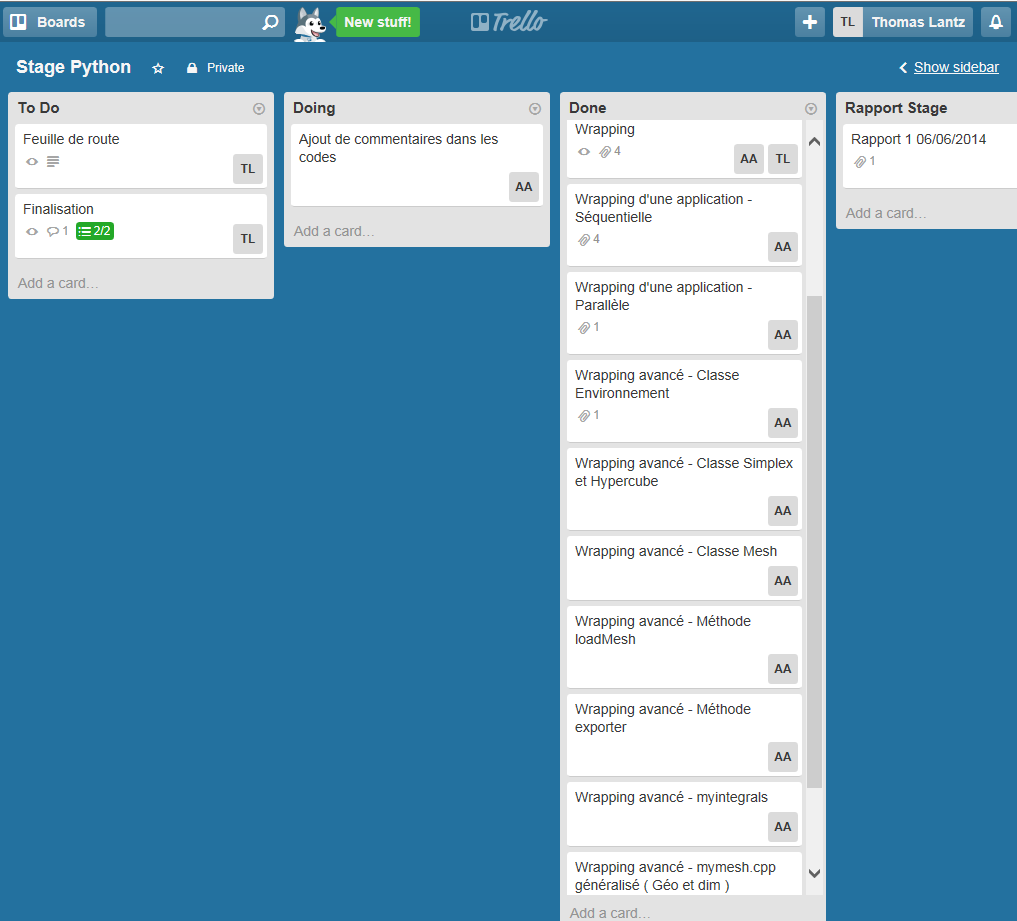
\includegraphics[scale=0.55]{1.png} 

\subsubsection{Github/Git}

Github est, quand à lui, une plateforme de stockage de projets en ligne. On crée, ou rejoint, un projet où l'on peut alors y stocker toutes sortes de documents, qui ne pourront être modifiés directement uniquement par les participants autorisés. 
Pour les autres, il est possible de récupérer une copie du projet, afin de travailler dessus et ensuite soumettre son travail qui pourra alors être intégré, ou non, au projet selon les résultats fournis.
\newline

Github utilise, pour la gestion des fichiers, Git, qui est un gestionnaire de versions, c'est à dire un programme permettant de stocker et gérer l'ensemble des versions de chaque fichiers. On peut ainsi à tout moment récupérer des versions d'un fichier antérieur à celui que l'on possède actuellement, ou même diviser un fichier sur deux "branches" distinctes, les modifier de manière différentes, et ensuite regrouper toutes ces modifications dans un seul fichier, tout en conservant bien sur toutes versions des 2 fichiers.\\

Pour se faire, on utilisera toute un liste de commandes assez similaire à celle du bash précédé de la commande git.

\subsubsection{Cmake}

CMake (ou cross plateform make) est, comme son nom l'indique, un programme de construction multi-plateforme, qui peut agir de pair avec la commande make. 
\newline

Grâce à des fichiers de configuration, appelés CMakeLists.txt, CMake permet de configurer différents objets comme des fichiers de code ou des exécutables et de générer les MakeFile associés selon ce que l'on a demandé dans les fichiers de configurations. Suite à leurs créations par ce procédé, on peut alors utiliser la commande make, afin d'appliquer les différentes instructions de compilation présentes dans ces fichiers.

\subsection{Feel++}

Feel++ est la librairie que l'on veut ici wrapper au cours de ce stage. Elle a été créer sur la base du langage C++ et son utilité se trouve dans la résolution de systèmes d'équations différentielles partiels à partir de méthodes mathématiques, comme la méthode des éléments finis ou la méthode de Galerkin par exemple.\\

On peut ainsi choisir un espace de définition, générer un espace d'interpolation ainsi qu'un maillage, définir les expressions des équations différentielles pour ensuite résoudre l'équation et récupérer enfin le résultat dans un fichier, que l'on pourra alors afficher avec Paraview, tout cela grâce au différentes méthodes de Feel++.

\section{Wrapping Python}
Après cette rapide présentation du sujet et des outils, nous allons pouvoir entrer dans le vif du sujet, en explicitant dans cette partie, le travail effectué pendant ces 2 mois et introduire de cette façon le manière dont j'ai procédé pour créer une librairie Python, ainsi que les difficultés que j'ai pu rencontré à chaque étape.
\newline

Tous les exemples traités sont présents intégralement dans l'annexe en fin de rapport.
\subsection{Introduction}

Commençons par introduire brièvement le principe de ce stage, c'est à dire en quoi consiste le wrapping Python.\\

Le wrapping Python consiste à générer une librairie à partir d'objets déjà implémentés en C++, comme les classes ou des méthodes par exemple, qui sera alors compréhensible, et donc utilisable par Python. Pour se faire, il existe des librairies déjà existantes permettant le partage entre ces 2 langages de programmation. Citons ici deux des exemples les plus connus et utilisés : Boost.Python et SWIG.\\ 

Chacune d'entre elles a ses avantages et inconvénients que l'on peut retrouver dans le lien suivant : \\
\url{https://dev.lsstcorp.org/trac/wiki/SwigVsBoostPython}
\vspace{0.5 cm}

On choisira donc ici Boost.Python plutôt que SWIG notamment par sa facilité à utiliser et gérer tout ce que porte aux pointeurs et aux références d'objets, grâce aux boost$::$shared\_ptr dont on parlera plus en détail plus tard.

\subsection{Boost.Python}
Après cette petite introduction, nous allons présenter plus en détail l'outil le plus important de ce stage, qui nous permettra de mettre en place les différentes librairies Python à partir du code Feel++ :  Boost.Python.
\newline

Boost.Python est une librairie C++ qui permet de transposer du code entre le C++ et Python. Elle permet en effet de récupérer des classes et méthodes déjà présentes en C++ afin de définir directement, à partir de leur définition, un équivalent en Python. 
\newline

Pour se faire, on utilisera alors la syntaxe suivante que l'on placera dans un fichier qu'on compilera afin de créer la bibliothèque :

\begin{lstlisting}
#include <boost/python.hpp>
#include <mpi4py/mpi4py.h>

BOOST_PYTHON_MODULE("libName")
{
 if (import_mpi4py()<0) return ;
 .....
 .....
}
\end{lstlisting}

avec "Name" le nom de la librairie voulue que l'on fera précéder d'un préfixe lib et à l'intérieur des accolades les classes et méthodes que l'on veut importer dans notre libraire Python avec une syntaxe qui serra présenter plus en détail pour chaque type d'objet. On utilise également la méthode import\_mpi4py()afin de vérifier que MPI est bien initialisé dans le script Python à partir du module mpi4py.
\newline

Il ne nous reste plus qu'à donner l'information à CMake qu'il doit compiler ce fichier en créant une librairie Python. Il suffit pour cela d'adopter le code suivant : 
\begin{lstlisting}
if(FEELPP_ENABLE_PYTHON)

add_library("Name" SHARED fichier.cpp)
target_link_libraries("Name" feelpp ${FEELPP_LIBRARIES})

endif()
\end{lstlisting}

On pourra remarquer qu'ici on utilise uniquement le nom de la librairie sans le préfixe lib devant, ainsi que l'utilisation d'une option nommé FEEL\_ENABLE\_PYTHON rajouté dans FindFeelpp.cmake afin de gérer si l'on veut ou non compiler ce fichier. 
\newline

On a alors créé la librairie associée aux méthodes et classes placées dans le BOOST\_PYTHON\_MODULE et il nous suffit de l'appeler comme n'importe quel autre module dans un script Python, comme suivant :
\begin{lstlisting}
#!/usr/bin/python

from mpi4py import MPI
import libName

t=libName.testFunction()
\end{lstlisting}

\subsection{Classes}
Commençons par voir comment wrapper les différents type de classes possibles.
Le wrapping de classe est utilisé principalement pour deux raisons : \\
- Création d'un objet du type de la classe wrappée et utilisation des méthodes associées. \\
- Récupération et définition d'un type de retour non connu (classes et instance définies en C++) par Python afin de pouvoir stocker les résultats dans des objets Python. \\

La syntaxe de base est la suivante:
\begin{lstlisting}
class_<"info\_sur\_la\_classe">("Name",init<arg>());
\end{lstlisting}
avec :\\
- info\_sur\_la\_classe qui correspond au nom de la classe que l'on veut récupérer ainsi qu'à une suite d'options que l'on peut rajouter, comme l'utilisation des pointeurs avec cette classe ou le méthode de création d'objet dynamique avec return\_value\_policy<T>, que l'on verra plus tard.\\
- Name qui correspond au nom de la classe Python associé à la classe C++ wrappé.\\
- init<arg>() si l'on veut ajouter un constructeur avec arg la liste des arguments prise par le constructeur en C++ que l'on veut récupérer. Si l'on n'en désire pas, on utilisera no\_init.\\

\subsubsection{Wrapping de classes simples}
Les classes simples sont les classes qui ne possèdent pas de template lors de leurs définitions. Prenons comme exemple la classe Environment, dont l'un des constructeurs est systématiquement utilisé à chaque début de programme, et qui est définie de la sorte :
\begin{lstlisting}
namespace Feel 
{
namespace detail
{
class Environment : boost::noncopyable
{
 ...
}
}
}
\end{lstlisting}
On veut donc pouvoir récupérer cette classe ainsi que son constructeur afin de pouvoir l'utiliser dans nos script Python. 
\newline

Pour cela, il suffit d'utiliser la syntaxe suivante :
\begin{lstlisting}
class_<Feel::detail::Environment,boost::noncopyable>("Environment",no_init);
\end{lstlisting}

On donne ainsi:\\
- la classe à wrapper, ici Feel$::$detail$::$Environment. \\
- boost$::$noncopyable par définiton de Environment. \\
- le nom associé à l'objet Python , ici Environment. \\

boost$::$noncopyable permet ici de déclarer private l'ensemble des fonctions de copies de la classe. Les définir private de cette manière rend l'action plus explicite et permet notamment de prévenir la classe ou des classes amies d'appeler ces méthodes. 
boost$::$noncopyable est ici indiqué lors du wrapping pour prévenir Python des propriétés associées de la classe.\\

C'est notamment l'un des paramètres que l'on peut placer ici entre les crochets définissant la classe wrappée. On verra quelques autres paramètres, servant également à définir la classe, que l'on peut également placé à la suite.

\subsubsection{Wrapping de classes avec templates}

Les classes avec templates causent elles un peu plus de soucis pour le wrapping. 
En effet, le Python étant un langage interprété et non compilé, l'utilisation de template est impossible et il faut donc remplir à chaque wrapping d'une classe les templates avec des valeurs particulières. Cela créer une barrière nous empêchant alors de transmettre du code générique au nouveau module Python.
\newline

Afin d'illustrer ces propos, prenons la classe Mesh qui s'occupe de générer les maillages et qui est définie de la sorte :
\begin{lstlisting}
template<typename GeoShape, typename T=double, int Tag=0>
class Mesh
{
 ...
}
\end{lstlisting}

On voit bien que Mesh nécessite un type d'élément du maillage en tant que templates et on ne peut pas simplement écrire :
\begin{lstlisting}
class_<Feel::Mesh<GeoShape>,boost::noncopyable>("Mesh",init<>())
\end{lstlisting}

En effet, l'écrire ainsi provoquera une erreur à la compilation, GeoShape étant un type général définit dans un template et Boost.Python ne permet pas de générer du code templaté, comme le Python ne possède pas d'équivalent à cela.

Il nous faut donc choisir un type, ici soit Simplex, soit Hypercube. Malheureusement, ces 2 types sont également liés à des templates par rapport à leurs dimensions. On doit de même définir les valeurs de ces dimensions si l'on veut récupérer un type d'objet en Python.
\newline

Ainsi pour avoir un maillage composé de triangles (Simplex de dimension 2), il faut écrire :
\begin{lstlisting}
class_<Feel::Mesh<Feel::Simplex<2>>,boost::noncopyable>("Mesh",init<>())
\end{lstlisting}

De même, si l'on veut un maillage composé de cubes (Hypercube de dimension 3), cela nous donne :
\begin{lstlisting}
class_<Feel::Mesh<Feel::Hypercube<3>>,boost::noncopyable>("Mesh",init<>())
\end{lstlisting}

On peut déjà entrevoir ici un des problèmes du wrapping Python, avec l'obligation de définir tous les templates pour des valeurs données, qui s'accentuera encore un peu quand il faudra appliquer des méthodes sur des objets templatés mais ce sera le sujet d'une partie suivante. On essayera également de corriger au mieux ce problème un peu plus loin.

\subsection{Méthodes}

Après ce bref aperçu sur le wrapping de classe, passons à celui des méthodes. On retrouve ici plus de cas différents que pour les classes, mais la syntaxe est la même pour toute.
\newline
Si la méthode appartient à une classe A par exemple et s'applique sur un objet instancié, on a alors :
\begin{lstlisting}
class_<A>("A",no_init)
.def("exe1",A::exe);
\end{lstlisting}

Si la méthode est virtual ou static, et est donc une méthode de classe, il suffit d'ajouter :
\begin{lstlisting}
class_<A>("A",no_init)
.def("exe1",A::exe)
.staticmethod("exe1");
\end{lstlisting}

Enfin si la méthode est libre, on a : 
\begin{lstlisting}
def("exe1",exe);
\end{lstlisting}

avec exe1 le nom que prendra la définition de notre méthode en Python, suivi ensuite de l'emplacement de cette méthode dans notre code Feel++.
\newline

\subsubsection{Wrapping de méthodes simples}

Commençons par le cas de base : les méthodes simples. Ce sont les fonctions sans templates présents ni dans les arguments ni dans le type de retour.
Pour ses méthodes là, il suffit d'appliquer la syntaxe présentée plus haut.\\

Par exemple, avec la méthode printMa1 définie par :
\begin{lstlisting}
void printMa1(integrate_return_type::value_type m)
{
 	std::cout << m << std::endl;
}
\end{lstlisting}

Il nous suffit alors d'écrire:
\begin{lstlisting}
def("printSol",,printMa1);
\end{lstlisting}

De même avec la méthode worldComm dans la classe Environment présentée avant, on a alors :
\begin{lstlisting}
class_<Feel::detail::Environment,boost::noncopyable>("Environment",no_init)
	.def("worldComm",&Feel::detail::Environment::worldComm,return_value_policy<copy_non_const_reference>())
.staticmethod("worldComm");
\end{lstlisting}

Il ne faut pas oublier de wrapper un objet du type de retour, si ce n'est pas un type simple (int,char,....) ou un type appartenant à Python (boost$::$python$::$list,..).

Ainsi pour l'exemple précédent, il faut indiquer à quoi correspond le type d'objet WorldComm de la façon suivante :
\begin{lstlisting}
class_<WorldComm>("WorldComm,init<>());
\end{lstlisting} 

On peut également observer ici deux nouvelles commandes :\\

- return\_value\_policy<T> qui permet d'indiquer à Python comment la méthode nouvellement construite doit fabriquer l'objet renvoyé. Ainsi, ici on construit l'objet de type WorlComm par référence. Il existe également d'autres paramètres pour obtenir des passages par valeurs ou par copie par exemple.\\

- staticmethod qui indique à Python que la méthode est définie statiquement.\\

Bien que ce soit le cas le plus simple, on peut déjà commencer à y rencontrer une petite difficulté, qui sera également présente dans tous les autres cas, de par la présence de pointeur dans les méthodes.\\
En effet, en Python la notion de pointeur n'est pas présente naturellement comme en C++ et quand on doit donner un $char**$ à une méthode wrappée, ce n'est pas possible directement.\\

Pour contrer ce problème, j'ai entamé pas mal de tests comme la création d'une classe entière avec un $char**$ comme argument ou de définir une classe équivalente à ce pointeur. De là sont sortis les deux solutions que l'on utilise suivant le cas rencontré :\\

- Pointeur sur un type de base : Dans ce cas, on va écrire une méthode, qui à partir d'une liste Python, va créer un $char**$, appellera la méthode voulue avec,  puis libérera la mémoire utilisée. C'est cette méthode que l'on wrappera alors en Python et qu'on utilisera à la place de la méthode initiale.\\

Par exemple pour l'appel d'une méthode test comme suivant :
\begin{lstlisting}
int test(int argc,char** argv)
\end{lstlisting}

On écrit une méthode comme suivant :
\begin{lstlisting}
void wrap(boost::python::list argv)
{
	int argc=boost::python::len(argv);
	char** pyarg=new cahr* [argc+1];
	boost::python::stl_imput_iterator<std::string> gegin(argv), end;
	int i=0;	
	while(begin != end)
	{
		pyarg[i]=strdup((*begin).c_str());
		begin++;
		i++;
	}
	pyarg[argc]=NULL;
	test(argc,pyarg);
	for(int i=0;i<argc;i++)
		delete pyarg[i];
	delete[] pyarg;
}	
\end{lstlisting}

Il ne reste alors plus qu'à la wrapper :
\begin{lstlisting}
def("main",test);
\end{lstlisting}

- Pointeur sur une classe : ici, on va travailler sur le wrapping de classes. En effet, si l'on veut appeler une méthode avec comme argument un pointeur sur un objet de type A, il y a de fortes chances que l'on ai déjà wrapper la classe A. 
Il suffit alors d'ajouter après avoir donné le type,  que cet objet peut également exister en temps que pointeur avec boost$::$shared\_ptr, de la sorte :
\begin{lstlisting}
class_<A,boost::shared_ptr<A>>("A",no_init)
\end{lstlisting}

On utilise ici boost$::$shared\_ptr, pour définir les types affiliés au pointeur, de par le fait que ces pointeurs sont directement liés à la librairie Boost, et sont donc compatibles avec la librairie Boost.Python, aussi issu de Boost.

\subsubsection{Wrapping de méthodes avec paramètres par défaut}

Les méthodes possédant des arguments par défaut se comportent exactement comme les méthodes associées sans arguments par défaut au niveau du wrapping. Cependant,  si on se contente de les wrapper telles quelles, Python va perdre la valeur des arguments par défaut, et on ne pourra alors plus appeler celles-ci simplement avec les arguments non définis.\\
On va pour corriger cela devoir redéfinir des sous-méthodes qui seront wrappées afin de prendre la place de la méthode principale : \\

Afin d’illustrer cela, prenons la méthode suivante comme exemple :
\begin{lstlisting}
template<typename MeshType>
boost::tuple<mpl::size_t<MESH_ELEMENTS>,
	typename MeshTraits<MeshType>::location_element_const_iterator,
	typename MeshTraits<MeshType>::location_element_const_iterator>
boundaryelements(MeshType const& mesh,uint16_type entity_min_dim=0,uint16_type entity_max_dim=2)
{
 ...
}
\end{lstlisting}

On peut définir une méthode de la sorte qui va l'appeler, comme suivant :
\begin{lstlisting}
template<typename MeshType>
boost::tuple<mpl::size_t<MESH_ELEMENTS>,
	typename MeshTraits<MeshType>::location_element_const_iterator,
	typename MeshTraits<MeshType>::location_element_const_iterator>
boundaryelements_w(MeshType const& mesh)
{
 	return boundaryelements(mesh);
}
\end{lstlisting}

On obtient alors une méthode sans avoir d'arguments par défaut, il suffit alors de la wrapper de la même façon que les méthodes présentées avant.\\

Cependant, en utilisant cette technique, on perd totalement l'accès à la variable définie par défaut. 
Dans le cas où l'on veut maintenant pouvoir utiliser soit la méthode en gardant la valeur par défaut, soit en la modifiant, il faut procéder autrement : \\

- On peut créer des sous-méthodes possédant chacune les arguments liés aux paramètres que souhaitent conservés. Par exemple, avec l'exemple précédent, on peut définir  : 
\begin{lstlisting}
template<typename MeshType>
boost::tuple<mpl::size_t<MESH_ELEMENTS>,
	typename MeshTraits<MeshType>::location_element_const_iterator,
	typename MeshTraits<MeshType>::location_element_const_iterator>
f1(MeshType const& mesh)
{
return boudaryelements(mesh);
}

template<typename MeshType>
boost::tuple<mpl::size_t<MESH_ELEMENTS>,
	typename MeshTraits<MeshType>::location_element_const_iterator,
	typename MeshTraits<MeshType>::location_element_const_iterator>
f2(MeshType const& mesh,uint16_type entity_min_dim=0)
{
return boudaryelements(mesh,entity_min_dim);
}

template<typename MeshType>
boost::tuple<mpl::size_t<MESH_ELEMENTS>,
	typename MeshTraits<MeshType>::location_element_const_iterator,
	typename MeshTraits<MeshType>::location_element_const_iterator>
f1(MeshType const& mesh,uint16_type entity_min_dim=0,uint16_type entity_max_dim=2)
{
return boudaryelements(mesh,entity_min_dim,entity_max_dim);
}
\end{lstlisting}

On peut alors wrapper ses trois méthodes en indiquant un nom commun pour leurs définitions en Python, comme suivant :
\begin{lstlisting}
def("boundaryelements",f1);
def("boundaryelements",f2);
def("boundaryelements",f3);
\end{lstlisting}

De cette façon, quand on appellera la méthode boundaryelements en Python, selon les paramètres donnés en arguments, il choisira la fonction associée.\\

- On peut également, pour se faire, utiliser deux macros contenues dans cette librairie : BOOST\_PYTHON\_FUNCTION\_OVERLOADS et \\ BOOST\_PYTHON\_MEMBER\_FUNCTION\_OVERLOADS.\\

Ces deux macros servent à générer automatiquement des classes contenant les wrappings des différentes méthodes surchargées, la première servant pour les méthodes libres, la seconde pour les méthodes de classes ou d'instances. Elles deviennent vraiment intéressantes quand le nombre de surcharges d'une méthode commence à grimper (supérieur à trois).\\

Malheureusement, je n'ai pas pu les utiliser durant le stage, mais ce sont des macros qui pourraient se révéler très utiles pour le futur du wrapping du code.

\subsubsection{Wrapping de méthodes avec templates}

Avec les méthodes possédant des templates, on va se retrouver avec le même soucis qu'avec les classes templatées, c'est à dire que l'on va devoir définir des valeurs pour chacun des templates. Et cela va à nouveau nous causer pas mal de soucis.\\

En effet, si un argument utilise un objet du template, la méthode ne pourra être appeler qu'avec le choix que l'on aura fait lors du remplissage de celui-ci.\\

Prenons la méthode loadMesh définie de la sorte :
\begin{lstlisting}
boost::shared_ptr<Mesh<Simplex<2>>> loadMesh_w (Mesh<Simplex<2>>* mesh)
{
 return loadMesh(_mesh=mesh);
}
\end{lstlisting}

Si l'on wrappe la méthode telle qu'elle est actuellement, on ne pourra l'utiliser que pour des objets du type Mesh<Simplex<2>> ce qui ne représente qu'une petite partie des types possibles que l'on pourrait avoir ici.\\

Afin de wrapper de telles méthodes, il y a deux solutions :\\

On peut soit redéfinir comme précédemment une nouvelle méthode avec les champs du template remplacés par les valeurs voulues, et on se retrouve avec une méthode qui ne possède plus de template.\\
Ainsi, la méthode suivante :
\begin{lstlisting}
template<typename MeshType>
boost::shared_ptr<MeshType> unitSquare()
{
 ...
}
\end{lstlisting}
peut s'écrire de la façon suivante:
\begin{lstlisting}
boost::shared_ptr<Mesh<Simplex<2>>> unitSquare_w ()
{
return unitSquare();
}
\end{lstlisting}

Ou alors on peut directement définir les valeurs voulues pour les membres du templates lors de la définition de la fonction dans le BOOST\_PYTHON\_MODULE de la façon suivante :\\
Soit la fonction suivante :
\begin{lstlisting}
template<typename MeshType,int N>
void expo_w ( boost::shared_ptr<MeshType> m)
{
auto x=Exporter<MeshType,N>::New();
x->setMesh(m);
x->addRegions();
x->save();
}
\end{lstlisting}

On peut alors directement la wrapper ainsi:
\begin{lstlisting}
def("export",expo_w<Mesh<Simplex<2>>,1>);
\end{lstlisting}

Nous avons parlé pour l'instant uniquement des soucis avec des arguments de la méthode liés au template, mais le type de retour peut également nous amener son lot de problèmes.\\

En effet, comme on doit indiquer à Python le type de retour en définissant une classe dans la librairie, on ne peut pas le faire de manière générique en conservant les templates. Il faut également donner des valeurs aux différents templates lors de ces définitions, et cela peut poser problème lorsque les types deviennent assez longs et compliqués à modifier pour d'autres valeurs du template.\\
Voici par exemple le type de retour du constructeur de Pch :
\begin{lstlisting}
Feel::FunctionSpace<Mesh<Simplex<2>>,Feel::bases<Feel::Lagrange<1,Feel::Scalar,Feel::Continuous,Feel::PointSetEquiSpaced,0>>,double,Feel::Periodicity<Feel::NoPeriodicity>,Feel::mortars<Feel::NoMortar>>
\end{lstlisting}

On essayera dans la dernière partie de ce rapport de trouver une solution à ce problème grâce à certains outils et librairies existantes.

\subsubsection{Wrapping de BOOST\_PARAMETER\_FUNCTION}

L'utilisation de la macro BOOST\_PARAMETER\_FUNCTION permet de générer une méthode spécifique à partir du nom, du type de retour et des arguments donnés .En effet, pour appeler ce type de méthode, il faut nommer les champs d'arguments à remplir suivi de la valeur que l'on veut associer.\\
Voici un exemple d'une BOOST\_PARAMETER\_FUNCTION que l'on vu juste avant : la méthode loadMesh.

\begin{lstlisting}
BOOST_PARAMETER_FUNCTION(
    ( typename Feel::detail::mesh<Args>::ptrtype ), // return type
    loadMesh,    // 2. function name
    tag,           // 3. namespace of tag types
    ( required
      ( mesh, *)
        ) // 4. one required parameter, and
    ( optional
      ( filename, *( boost::is_convertible<mpl::_,std::string> ), option(_name="gmsh.filename").template as<std::string>() )
      ( desc, *,boost::shared_ptr<gmsh_type>() )  // geo() can't be used here as default !!
      .....
      .....
        )
    )
\end{lstlisting}
On peut alors l'appeler par exemple de la façon suivante : 
\begin{lstlisting}
auto mesh = loadMesh( _mesh=new Mesh<Simplex<2>> );
\end{lstlisting}

Afin de wrapper des méthodes de ce type, il existe des méthodes spécifiques présentées dans le lien suivant :\\
\url{http://www.boost.org/doc/libs/1_46_0/libs/parameter/doc/html/python.html}
\vspace{0.5 cm}

Pour expliquer brièvement la technique présentée, on construit à partir de la BOOST\_PARAMETER\_FUNCTION une méthode qui possède tous les arguments dans un template avec le type de retour. Il ne reste alors plus qu'à wrapper cette nouvelle méthode, afin de pouvoir l'utiliser de la même manière qu'en C++.\\

Malheureusement, je n'ai pas réussi à les appliquer et les mettre en œuvre au cours de mon stage.
En effet, j'ai tenté plusieurs essais sur des fonctions différentes, que sont loadMesh et exporter. Mais dans chacun de ces deux cas, et malgré les différentes tentatives, j'obtenais toujours une erreur m'indiquant qu'il ne pouvait trouver de méthodes correspondant à celle crée avec le template.\\

Je me suis alors rabattu sur une technique, voir plutôt une astuce, similaire à ce que j'ai utilisé jusqu'à présent. 
Pour cela, il suffit de créer une nouvelle méthode avec le même type de retour et les arguments que l'on veut utiliser, et simplement d'appeler la fonction défini par la BOOST\_PARAMETER\_FUNCTION.\\
En reprenant l'exemple précédent de loadMesh, on obtient :
\begin{lstlisting}
boost::shared_ptr<Mesh<Simplex<2>>> loadMesh_w (Mesh<Simplex<2>>* mesh)
{
 return loadMesh(_mesh=mesh);
}
\end{lstlisting}

Il suffit alors comme plus haut de wrapper cette nouvelle fonction et de l'utiliser dans notre script Python. Cependant, de part cette astuce, on perd la possibilité de pouvoir appeler la méthode originelle avec les champs et arguments voulus, modifiable à tout moment dans le script Python.

\subsection{Parallélisme}

MPI, donc l'exécution de programmes en parallèle, est déjà utilisé et implémenté dans la librairie Feel++, on peut se demander alors si l'on peut conserver cette fonctionnalité après le wrapping Python.\\

Comme on a pu le voir brièvement en début de cette partie, on ajoute deux lignes permettant l'initialisation et l'utilisation de MPI en Python.\\

- from mpi4py import MPI, qui se trouve au début du script Python, initialise automatiquement MPI à l'importation (à l'inverse de MPI en C++ qui demande une méthode pour son initialisation). La destruction se  fait aussi automatiquement à la fin du programme Python.\\

- if (import\_mpi4py()<0) return ; , quand à lui, se trouve au tout début de la définition du BOOST\_PYTHON\_MODULE, et permet de créer le module seulement si l'importation de mpi4py, et donc la présence de MPI, est réussite.\\

Ces 2 méthodes se trouvent dans la librairie mpi4py, que l'on retrouve aussi bien en C++ qu'en Python, et qui permet donc de lier ces 2 langages. Quand à la possibilité de paralléliser l'exécution des méthodes wrappées, l'utilisation de Boost.Python permet de conserver cette propriété pour tout les objets.\\

Il ne reste plus qu'a appeler le script Python avec MPI, de la même manière qu'en C++, c'est à dire : \\
\begin{lstlisting}
mpirun -np 4 ./Feelpp.py
\end{lstlisting}

Ce qui nous par exemple sur Paraview : \\

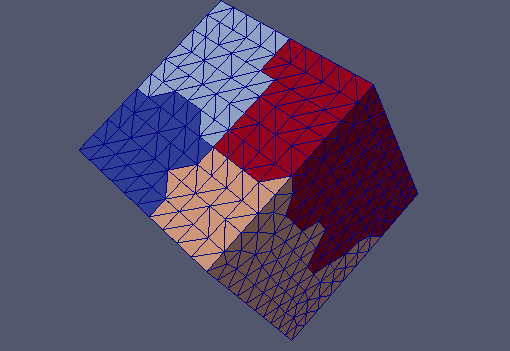
\includegraphics[scale=0.60]{MPI.png} 

\subsection{Trucs et Astuces}

On va, dans cette section, rapidement présenter quelques astuces facilitant le wrapping de classes et méthodes.

\subsubsection{Récupération du type de retour}

Wrapper le type de retour peut être particulièrement difficile, notamment quand il est remplacé par un typename dans la définition de la méthode et, qu'en plus de cela, il est composé de templates. On doit alors donner le type exact de retour avec les templates remplis pour pouvoir utiliser un objet de ce type.\\

C'est là qu'intervient une astuce, nommé "give bad to have good", dont l'idée m'est venu suite à une discussion sur le type de retour de la méthode integrate avec mes camarades de stage.

L'idée est donc de donner un type de base que l'on sait faux de toute façon, et attendre alors que la compilation nous renvoie alors l'erreur avec le type à récupérer. J'ai ainsi pu récupérer notamment des types comme le suivant qui serait en temps normal introuvable aussi rapidement : 

\begin{lstlisting}
typedef boost::tuples::tuple<mpl_::size_t<0ul>, boost::multi_index::detail::bidir_node_iterator<boost::multi_index::detail::ordered_index_node<boost::multi_index::detail::ordered_index_node<boost::multi_index::detail::ordered_index_node<boost::multi_index::detail::ordered_index_node<boost::multi_index::detail::ordered_index_node<boost::multi_index::detail::ordered_index_node<boost::multi_index::detail::ordered_index_node<boost::multi_index::detail::index_node_base<Feel::GeoElement3D<(unsigned short)3, Feel::Simplex<(unsigned short)3, (unsigned short)1, (unsigned short)3>, double>, std::allocator<Feel::GeoElement3D<(unsigned short)3, Feel::Simplex<(unsigned short)3, (unsigned short)1, (unsigned short)3>, double> > > > > > > > > > >, boost::multi_index::detail::bidir_node_iterator<boost::multi_index::detail::ordered_index_node<boost::multi_index::detail::ordered_index_node<boost::multi_index::detail::ordered_index_node<boost::multi_index::detail::ordered_index_node<boost::multi_index::detail::ordered_index_node<boost::multi_index::detail::ordered_index_node<boost::multi_index::detail::ordered_index_node<boost::multi_index::detail::index_node_base<Feel::GeoElement3D<(unsigned short)3, Feel::Simplex<(unsigned short)3, (unsigned short)1, (unsigned short)3>, double>, std::allocator<Feel::GeoElement3D<(unsigned short)3, Feel::Simplex<(unsigned short)3, (unsigned short)1, (unsigned short)3>, double> > > > > > > > > > >, boost::tuples::null_type, boost::tuples::null_type, boost::tuples::null_type, boost::tuples::null_type, boost::tuples::null_type, boost::tuples::null_type, boost::tuples::null_type> elements_return_type; 
\end{lstlisting}

Il ne reste plus qu'à utiliser un typedef comme ci-dessus pour pouvoir l'utiliser efficacement dans le code.

\section{Généralisation du Wrapping Python}

Pour terminer, après cette présentation de différentes méthodes pour wrapper différents types d'objets, je finirai par le résultat le plus important de ce stage.
En effet, tout les résultats présentés jusqu'à maintenant étaient des wrappings spécifiques à des exemples particuliers, notamment par des dimensions données. Si l'on veut maintenant changer une dimension, par exemple la dimension des éléments du maillage, il faut absolument tout recommencer et tout réécrire avec ce nouveau paramètre, ce qui peut être fastidieux si le nombre de paramètres et le nombre de valeurs par paramètres augmentent.

On veut donc généraliser les méthodes primordiales de Feelpp pour toutes les valeurs possibles et c'est que je vais vous présenter maintenant

\subsection{Boost.Preprocessor}

Afin de pouvoir généraliser le wrapping des classes et méthodes possédant un template, nous allons utiliser la bibliothèque Boost.Preprocessor.\\

Boost.Preprocessor est une librairie contenant toutes sortes de macros et permettant de faire de la métaprogrammation, c'est à dire générer du code à partir de ces macros, qui seront alors utilisées lors de la compilation.\\

Si l'on veut voir le code tel qu'il est après application des macros, il suffit de trouver le fichier portant le même nom que celui contenant les macros suivi de l'extension .i, que l'on obtient de la manière suivante : 
\begin{lstlisting}
make - j 4 libPyFeelpp.i
\end{lstlisting}

Par exemple, pour le fichier libPyFeelp.cpp que l'on regardera plus tard, on va regarder le fichier nommé libPyFeelp.cpp.i  .\\
On le trouve généralement en suivant le chemin suivant $CMakeFiles/"nom\_du\_fichier"/$ à partir du dossier contenant les exécutables.\\

Afin de générer le code, nous allons principalement utiliser la macro suivante :
\begin{lstlisting}
BOOST_PP_REPEAT(n,X,Y)
\end{lstlisting}
qui permet de répéter la méthode Y suivant la macro X avec une variable comprise entre 0 et n-1. Nous verrons des exemples de son utilisation dans la partie suivante.\\

On s'intéressera alors d'autres macros de cette librairie pour essayer de récupérer des méthodes plus compliquées à wrapper.

\subsection{La librairie Feelpp}

Avec tout les outils présentés jusqu'à maintenant, ainsi que tout le travail déjà effectué sur les méthodes et classes de la librairie Feel++, on aimerait pouvoir créer un module Python possédant une généralisation des objets et fonctions les plus utiles de Feelpp afin de pouvoir modifier les scripts Python à volonté sans avoir à recréer une nouvelle librairie pour chaque variation, comme on le faisait jusqu'à présent.\\

Pour illustrer cette méthode, prenons l'exemple de la définition des maillages pour tout type de géométrie (Hypercube ou Simplex) et pour toutes les dimensions possibles.\\

On va commencer par définir les macros que l'on utilisera avec les BOOST\_PP\_REPEAT de la façon suivante :
\begin{lstlisting}
#define SIMPLEX(_,n,type) type<n+1,1>("Simplex");
#define HYPERCUBE(_,n,type) type<n+1,1>("Hypercube");
\end{lstlisting}

A partir de celle-ci, implémentons les méthodes, contenant le code définissant le wrapping des objets voulus, et qui seront appelées sur les macros précédentes.
\begin{lstlisting}
    template <int n,int N>
void def_wrapper (std::string s)
{    
    std::ostringstream f;
    std::ostringstream g;
    if(s.compare("Simplex")==0)
    {
        f<<"Simplex"<<n;
        g<<"MeshS"<<n;
        class_<Feel::Simplex<n>>(f.str().c_str(),init<>());
        class_<Feel::Mesh<Simplex<n>>,boost::shared_ptr<Feel::Mesh<Simplex<n>>>,boost::noncopyable>(g.str().c_str(),init<>())
            .def("new",&Feel::Mesh<Simplex<n>>::New)
            .staticmethod("new");
        def("loadMesh",loadMesh_w<Mesh<Simplex<n>>>);
        def("export",expo_w<Mesh<Simplex<n>>,N>);
    }
    else if(s.compare("Hypercube")==0)
    {
        f<<"Hypercube"<<n;
        g<<"MeshH"<<n;   
        class_<Feel::Hypercube<n>>(f.str().c_str(),init<>());
        class_<Feel::Mesh<Hypercube<n>>,boost::shared_ptr<Feel::Mesh<Hypercube<n>>>,boost::noncopyable>(g.str().c_str(),init<>())
            .def("new",&Feel::Mesh<Hypercube<n>>::New)
            .staticmethod("new");
        def("loadMesh",loadMesh_w<Mesh<Hypercube<n>>>);
        def("export",expo_w<Mesh<Hypercube<n>>,N>);
    }
}
\end{lstlisting}

Il ne nous reste plus qu'à utiliser la macro présentée précédemment : BOOST\_PP\_REPEAT.
\begin{lstlisting}
BOOST_PP_REPEAT(3,SIMPLEX,def_wrapper)
BOOST_PP_REPEAT(3,HYPERCUBE,def_wrapper)
\end{lstlisting}

Cela est équivalent au code suivant :
\begin{lstlisting}
def_wrapper<1,1>("Simplex");
def_wrapper<2,1>("Simplex");
def_wrapper<3,1>("Simplex");
def_wrapper<1,1>("Hypercube");
def_wrapper<2,1>("Hypercube");
def_wrapper<3,1>("Hypercube");
\end{lstlisting}

Il ne nous reste alors qu'à suivre cette procédure pour les autres éléments comprenant des variables à définir pour le wrapping (en l'occurrence ici, la classe Pch ainsi que ces méthodes associées). Il ne nous reste alors qu'à wrapper l'ensemble des petites fonctions présentes dans Feelpp, comme les méthodes id, idv ou gradv qui l'on pourra alors utiliser pour générer toutes les expressions que l'on voudra dans nos script Python.\\

Pour se faire, il faut déjà trouver ces fonctions. En effet, elles sont déjà toutes définies à partir d’enchaînements de macros provenant de Boost.Preprocessor, ce n'est donc pas aussi facile que les méthodes présentées plus haut.\\
On récupère les types et les noms des méthodes de la façon suivante :
\begin{lstlisting}
#define VF_CLASS_DEF(_,OT)\
    VF_CLASS_DEF2 OT;

#define VF_CLASS_DEF2(O,T) \
     class_<Expr<BOOST_PP_CAT(expr_t,BOOST_PP_CAT(VF_OPERATOR_SYMBOL(O),VF_OP_TYPE_SUFFIX(T)))>>(BOOST_PP_STRINGIZE(BOOST_PP_CAT(expr_t,BOOST_PP_CAT(VF_OPERATOR_SYMBOL(O),VF_OP_TYPE_SUFFIX(T)))),no_init)

#define VF_METHODS_DEF(_,OT)\
    VF_METHODS_DEF2 OT;
    
#define VF_METHODS_DEF2(O,T)\
    def(BOOST_PP_STRINGIZE(BOOST_PP_CAT(VF_OPERATOR_SYMBOL(O),VF_OP_TYPE_SUFFIX(T))),Feel::vf::BOOST_PP_CAT(VF_OPERATOR_SYMBOL(O),VF_OP_TYPE_SUFFIX(T)))       
\end{lstlisting}

On utilise ici d'autres macros de Boost.Preprocessor :\\

- BOOST\_PP\_STRINGIZE qui permet de transformer en string l'argument donné. Ainsi BOOST\_PP\_STRINGIZE(Test) nous donne "Test" par exemple.\\

- BOOST\_PP\_CAT permet de concaténer les deux arguments que cette macro reçoit.\\

Les autres macros utilisées étant définis dans le fichier où sont définis toutes ces méthodes.

Grâce à une autre macro, déjà utilisée dans la définition de ces méthodes, on essaye de les intégrer à notre bibliothèque Python :
\begin{lstlisting}
BOOST_PP_LIST_FOR_EACH_PRODUCT(VF_CLASS_DEF,2,(VF_OPERATORS,VF_OPERATORS_TYPE))

BOOST_PP_LIST_FOR_EACH_PRODUCT(VF_METHODS_DEF,2,(VF_OPERATORS,VF_OPERATORS_TYPE))
\end{lstlisting}

On définit ainsi respectivement les différentes classes liées au type de retour de chaque méthode, puis les méthodes elles-même pour les intégrer dans notre module Python.\\

Voici donc une liste de ce qui est disponible actuellement dans ce module :\\
- Création de maillages avec les éléments Simplex et Hypercube pour les dimensions allant de un à trois.\\
- Création d'espaces d'interpolation de type Pch avec les dimensions variant de un à trois également.\\
- Récupération des différents types de maillages avec la méthode loadMesh.\\
- Exportation des divers maillages avec la méthode exporter (Soucis avec les maillages composés d'hypercube de dimension 2 et 3, aussi présent en C++) pour l'affichage avec Paraview.\\

\section{Conclusion et Futur}
Ceci conclut mon rapport portant sur mes travaux effectués sur le wrapping Python. On a ainsi pu voir comment wrapper les différents types de classes ou de méthodes qui nous sont proposés dans la librairie Feelpp.\\

Cela nous a permis de mettre en évidence différents soucis rencontrés lors des multiples exemples traités,  et notamment le fait que l'on ne peut pas wrapper génériquement les méthodes et classes possédant des templates.\\

C'est pour cela que l'on essaye alors de créer une librairie Python générale, qui nous permettra alors de pouvoir reproduire tout code de Feel++ en Python.\\

Voila où nous en sommes actuellement dans la création de ce module Python. Afin d'accomplir le but qui vient d'être exposé, il nous reste encore beaucoup de classes et de méthodes à wrapper, et notamment finir le travail entamé sur les méthodes propre à Feelpp en fin de stage mais qui n'a pas eu le temps d'aboutir.\\

De plus, il reste également quelques travaux de finition à faire sur ce qui a déjà été implémenté.
En effet, l'utilisation de la méthode loadMesh wrappée cause une erreur de segmentation lors de la destruction de l'objet construit à partir de cette méthode. Cela ne cause aucun soucis à l'utilisation de la méthode, mais c'est un petit soucis que l'on pourrait corriger.\\

Enfin, on a implémenté les objets de type Pch, cependant la possibilité de récupérer des éléments de ces espaces n'est pas encore mise en pratique de manière générale, vu la complexité de wrapper le type de retour. De ce fait, sans cela, on ne peut pas utiliser les autres méthodes afin de créer des expressions utilisées pour résoudre des équations différentielles.\\

De mon coté, ce stage m'a permis d'en apprendre plus dans divers domaines. Tout d'abord, j'ai pu en apprendre plus sur de nombreuses méthodes de Feelpp et donc sur le fonctionnement général de celui-ci.\\

De même, j'ai pu accroître mes connaissances sur les nombreuses facettes du wrapping Python, que j'avais légèrement aperçu lors des cours de Python ce semestre, grâce aux différentes recherches sur les librairies existantes ainsi que l'utilisation de Boost.Python.\\

Enfin l'utilisation des différents nouveaux outils,  ainsi que les conditions de travail du stage m'ont permis d'en apprendre plus sur le monde du travail, et d'améliorer mes connaissances et mes possibilités en programmation.

\newpage
\part{Annexes}
\section{Codes}

\subsection{Exemple myfunctionspace}

\subsubsection{Wrapping de la méthode test}
\begin{lstlisting}
int test (int argc,char** argv)
{
    for(int i=0;i<argc;i++)
         std::cout << argv[i] << std::endl;
    //Initialize Feel++ Environment
   
   /*
    Environment env( _argc=argc, _argv=argv,
                     _about=about( _name="myfunctionspace",
                                   _author="Feel++ Consortium",
                                   _email="feelpp-devel@feelpp.org" )  );
    */
    Environment env(argc,argv);
    

    //! [mesh]
    // create the mesh
    auto mesh = loadMesh(_mesh=new Mesh<Simplex<2>>);
    //! [mesh]

    //! [space]
    // function space \f$ X_h \f$ using order 2 Lagrange basis functions
    auto Xh = Pch<2>( mesh );
    //! [space]

    //! [expression]
    auto g = expr( soption(_name="functions.g"));
    auto gradg = grad<2>(g);
    //! [expression]

    //! [interpolant]
    // elements of \f$ u,w \in X_h \f$
    auto u = Xh->element( "u" );
    auto w = Xh->element( "w" );
    // build the interpolant of u
    u.on( _range=elements( mesh ), _expr=g );
    // build the interpolant of the interpolation error
    w.on( _range=elements( mesh ), _expr=idv( u )-g );

    // compute L2 norms
    double L2g = normL2( elements( mesh ), g );
    double H1g = normL2( elements( mesh ), _expr=g,_grad_expr=gradg );
    double L2uerror = normL2( elements( mesh ), ( idv( u )-g ) );
    double H1uerror = normH1( elements( mesh ), _expr=( idv( u )-g ),
                              _grad_expr=( gradv( u )-gradg ) );
    std::cout << "||u-g||_0 = " << L2uerror/L2g << std::endl;
    std::cout << "||u-g||_1 = " << H1uerror/H1g << std::endl;
     //! [interpolant]

    //! [export]
    // export for post-processing
    auto e = exporter( _mesh=mesh );
    // save interpolant
    e->add( "g", u );
    // save interpolant of interpolation error
    e->add( "u-g", w );

    e->save();
    //! [export]

            return 1;  
}
//! [all]


#include <boost/python.hpp>
#include <boost/python/stl_iterator.hpp>
#include <mpi4py/mpi4py.h>

// build an arguments recuperator from a Python object list to call the test method
void wrap( boost::python::list argv)
{
    int argc = boost::python::len(argv);
    std::cout << argc << std::endl ;
        
    char** pyarg =new char* [argc+1];
    boost::python::stl_input_iterator<std::string> begin(argv), end;
    int i=0;
    while (begin != end)
    {
        std::cout << *begin << std::endl ;
        pyarg[i] =strdup((*begin).c_str());
        begin++;
        i++;
    }
    pyarg[argc]=NULL;
    test(argc,pyarg);
    std::cout << "It's working !!!!" << std::endl; 
    for(int i=0;i<argc;i++)
        delete pyarg[i];
    delete[] pyarg;
}

//call the test method 
int main (int argc,char** argv)
{
    test(argc,argv);
}    


#include <boost/python.hpp>
using namespace boost::python;

// build the module, named libFunct, from previous methods
BOOST_PYTHON_MODULE(libFunct)
{
    if (import_mpi4py() <0) return ;
    def("test",test); 
    def("wrap",wrap);
    def("main",main);
   
}
\end{lstlisting}

\subsection{Exemple mymesh}
\subsubsection{Exemple à wrapper}
\begin{lstlisting}
Environment env( _argc=argc, _argv=argv,
                     _about=about( _name="mymesh" ,
                                   _author="Feel++ Consortium",
                                   _email="feelpp-devel@feelpp.org" ) );
    //! [load]
    // create a mesh with GMSH using Feel++ geometry tool
    auto mesh = loadMesh(_mesh=new  Mesh<Simplex<2>>);
    //! [load]

    //! [export]
    // export results for post processing
    auto e = exporter( _mesh=mesh );
    e->addRegions();
    e->save();
    //! [export]

\end{lstlisting}
\subsubsection{Définition du module : libPyMesh.cpp}
\begin{lstlisting}
#include <feel/feel.hpp>
#include <boost/python.hpp>
#include <boost/python/stl_iterator.hpp>
#include <mpi4py/mpi4py.h>

#include <boost/shared_ptr.hpp>
#include <boost/parameter/keyword.hpp>
#include <boost/parameter/preprocessor.hpp>
#include <boost/parameter/binding.hpp>
#include <boost/parameter/python.hpp>
#include <boost/python.hpp>
#include <boost/mpl/vector.hpp>

#include<feel/feelcore/environment.hpp>
#include<feel/feelfilters/loadmesh.hpp>
#include<feel/feelfilters/exporter.hpp>
#include<feel/feelfilters/detail/mesh.hpp>


using namespace boost::python;
using namespace Feel;

namespace py = boost::parameter::python;

// redefine exporter and loadMesh methods, created from a BOOST_PARAMETER_FUNCTION, into simple definition
 
    template<typename MeshType,int N>
void expo_w ( boost::shared_ptr<MeshType> m)
{
    auto x=Exporter<MeshType,N>::New();
    x->setMesh(m);
    x->addRegions();
    x->save();
}

boost::shared_ptr<Mesh<Simplex<2>>> loadMesh_w (Mesh<Simplex<2>>* mesh)
{
    return loadMesh(_mesh=mesh);
}

// creation of the libPyMesh library, that we will use in the Python script 

BOOST_PYTHON_MODULE(libPyMesh)
{

    if (import_mpi4py()<0) return ;

// definition of the Environment object and methods and classes link to it 
    class_<Feel::detail::Environment,boost::noncopyable>("Environment", init<boost::python::list>()) 
        .def("worldComm",&Feel::detail::Environment::worldComm,return_value_policy<copy_non_const_reference>())
        .staticmethod("worldComm");

    class_<WorldComm>("WorldComm",init<>());


// definition of the geometrical object (Simplex and Hypercube) and of the Mesh class 
    class_<Feel::Simplex<2>>("Simplex",init<>())
        .def("dim",&Feel::Simplex<2>::dimension);

    class_<Feel::Hypercube<2>>("Hypercube",init<>())
        .def("dim",&Feel::Hypercube<2>::dimension);



    class_<Feel::Mesh<Feel::Simplex<2>>,boost::shared_ptr<Feel::Mesh<Feel::Simplex<2>>>,boost::noncopyable>("Mesh",init<>())
        .def("new",&Feel::Mesh<Simplex<2>>::New)
        .staticmethod("new")
        .def("clear",&Feel::Mesh<Simplex<2>>::clear);


//definition of the loadMesh and exporter methods with functions define before 
    def("loadMesh",loadMesh_w);

    class_<ExporterEnsightGold<Mesh<Simplex<2>>,1>>("Exporter",init<WorldComm>())
        .def("setMesh",&Exporter<Mesh<Simplex<2>>>::setMesh) 
        .def("addRegions",&Exporter<Mesh<Simplex<2>>>::addRegions)
        .def("save",&ExporterEnsightGold<Mesh<Simplex<2>>,1>::save);


    def("export",expo_w<Mesh<Simplex<2>>,1>);
}
\end{lstlisting}
\subsubsection{Script Python : mymesh.py}
\begin{lstlisting}
## to move into the folders where Python libraries are created

#!/usr/bin/python

from mpi4py import MPI
import libPyMesh
import sys

z=libPyMesh.Environment(sys.argv)
s=libPyMesh.Simplex()
m=libPyMesh.Mesh.new()
l=libPyMesh.loadMesh(m)
w=libPyMesh.Environment.worldComm()

x=libPyMesh.export(l);
\end{lstlisting}

\subsection{Exemple myintegrals}
\subsubsection{Exemple à wrapper}
\begin{lstlisting}
Environment env( _argc=argc, _argv=argv,
                     _about=about( _name="myintegrals" ,
                                   _author="Feel++ Consortium",
                                   _email="feelpp-devel@feelpp.org" ) );

    /// [mesh]
    // create the mesh (specify the dimension of geometric entity)
    auto mesh = loadMesh( _mesh=new Mesh<Simplex<2>> );
    /// [mesh]

    /// [expression]
    // our function to integrate
    auto g = expr( soption(_name="functions.g") );
    /// [expression]

    /// [integrals]
    // compute integral of f (global contribution)
    auto intf_1 = integrate( _range = elements( mesh ),
                                 _expr = g ).evaluate();

    // compute integral f on boundary
    auto intf_2 = integrate( _range = boundaryfaces( mesh ),
                             _expr = g ).evaluate();

    // compute integral of grad f (global contribution)
    auto grad_g = grad<2>(g);
    auto intgrad_f = integrate( _range = elements( mesh ),
                                _expr = grad_g ).evaluate();

    // only the process with rank 0 prints to the screen to avoid clutter
    if ( Environment::isMasterRank() )
        std::cout << "int_Omega " << g << " = " << intf_1  << std::endl
                  << "int_{boundary of Omega} " << g << " = " << intf_2 << std::endl
                  << "int_Omega grad " << g << " = "
                  << "int_Omega  " << grad_g << " = "
                  << intgrad_f  << std::endl;
\end{lstlisting}
\subsubsection{Définition du module : libPyInteg.cpp}
\begin{lstlisting}
#include <feel/feel.hpp>
#include <boost/python.hpp>
#include <boost/python/stl_iterator.hpp>
#include <mpi4py/mpi4py.h>

#include <boost/shared_ptr.hpp>
#include <boost/parameter/keyword.hpp>
#include <boost/parameter/preprocessor.hpp>
#include <boost/parameter/binding.hpp>
#include <boost/parameter/python.hpp>
#include <boost/python.hpp>
#include <boost/mpl/vector.hpp>

#include<feel/feelcore/environment.hpp>
#include<feel/feelfilters/loadmesh.hpp>
#include<feel/feelfilters/exporter.hpp>
#include<feel/feelfilters/detail/mesh.hpp>

// retrieval of complicated return types with the "give bad type to have the good one" trick  

typedef boost::tuples::tuple<mpl_::size_t<0ul>, boost::multi_index::detail::bidir_node_iterator<boost::multi_index::detail::ordered_index_node<boost::multi_index::detail::ordered_index_node<boost::multi_index::detail::ordered_index_node<boost::multi_index::detail::ordered_index_node<boost::multi_index::detail::ordered_index_node<boost::multi_index::detail::ordered_index_node<boost::multi_index::detail::ordered_index_node<boost::multi_index::detail::index_node_base<Feel::GeoElement3D<(unsigned short)3, Feel::Simplex<(unsigned short)3, (unsigned short)1, (unsigned short)3>, double>, std::allocator<Feel::GeoElement3D<(unsigned short)3, Feel::Simplex<(unsigned short)3, (unsigned short)1, (unsigned short)3>, double> > > > > > > > > > >, boost::multi_index::detail::bidir_node_iterator<boost::multi_index::detail::ordered_index_node<boost::multi_index::detail::ordered_index_node<boost::multi_index::detail::ordered_index_node<boost::multi_index::detail::ordered_index_node<boost::multi_index::detail::ordered_index_node<boost::multi_index::detail::ordered_index_node<boost::multi_index::detail::ordered_index_node<boost::multi_index::detail::index_node_base<Feel::GeoElement3D<(unsigned short)3, Feel::Simplex<(unsigned short)3, (unsigned short)1, (unsigned short)3>, double>, std::allocator<Feel::GeoElement3D<(unsigned short)3, Feel::Simplex<(unsigned short)3, (unsigned short)1, (unsigned short)3>, double> > > > > > > > > > >, boost::tuples::null_type, boost::tuples::null_type, boost::tuples::null_type, boost::tuples::null_type, boost::tuples::null_type, boost::tuples::null_type, boost::tuples::null_type> elements_return_type; 

typedef boost::tuples::tuple<mpl_::size_t<0ul>, boost::multi_index::detail::bidir_node_iterator<boost::multi_index::detail::ordered_index_node<boost::multi_index::detail::ordered_index_node<boost::multi_index::detail::ordered_index_node<boost::multi_index::detail::index_node_base<Feel::GeoElement3D<(unsigned short)3, Feel::Simplex<(unsigned short)3, (unsigned short)1, (unsigned short)3>, double>, std::allocator<Feel::GeoElement3D<(unsigned short)3, Feel::Simplex<(unsigned short)3, (unsigned short)1, (unsigned short)3>, double> > > > > > >, boost::multi_index::detail::bidir_node_iterator<boost::multi_index::detail::ordered_index_node<boost::multi_index::detail::ordered_index_node<boost::multi_index::detail::ordered_index_node<boost::multi_index::detail::index_node_base<Feel::GeoElement3D<(unsigned short)3, Feel::Simplex<(unsigned short)3, (unsigned short)1, (unsigned short)3>, double>, std::allocator<Feel::GeoElement3D<(unsigned short)3, Feel::Simplex<(unsigned short)3, (unsigned short)1, (unsigned short)3>, double> > > > > > >, boost::tuples::null_type, boost::tuples::null_type, boost::tuples::null_type, boost::tuples::null_type, boost::tuples::null_type, boost::tuples::null_type, boost::tuples::null_type> boundaryelements_return_type;

typedef boost::tuples::tuple<mpl_::size_t<1ul>, boost::multi_index::detail::bidir_node_iterator<boost::multi_index::detail::ordered_index_node<boost::multi_index::detail::index_node_base<Feel::GeoElement2D<(unsigned short)3, Feel::Simplex<(unsigned short)2, (unsigned short)1, (unsigned short)3>, Feel::SubFaceOf<Feel::GeoElement3D<(unsigned short)3, Feel::Simplex<(unsigned short)3, (unsigned short)1, (unsigned short)3>, double> >, double>, std::allocator<Feel::GeoElement2D<(unsigned short)3, Feel::Simplex<(unsigned short)2, (unsigned short)1, (unsigned short)3>, Feel::SubFaceOf<Feel::GeoElement3D<(unsigned short)3, Feel::Simplex<(unsigned short)3, (unsigned short)1, (unsigned short)3>, double> >, double> > > > >, boost::multi_index::detail::bidir_node_iterator<boost::multi_index::detail::ordered_index_node<boost::multi_index::detail::index_node_base<Feel::GeoElement2D<(unsigned short)3, Feel::Simplex<(unsigned short)2, (unsigned short)1, (unsigned short)3>, Feel::SubFaceOf<Feel::GeoElement3D<(unsigned short)3, Feel::Simplex<(unsigned short)3, (unsigned short)1, (unsigned short)3>, double> >, double>, std::allocator<Feel::GeoElement2D<(unsigned short)3, Feel::Simplex<(unsigned short)2, (unsigned short)1, (unsigned short)3>, Feel::SubFaceOf<Feel::GeoElement3D<(unsigned short)3, Feel::Simplex<(unsigned short)3, (unsigned short)1, (unsigned short)3>, double> >, double> > > > >, boost::tuples::null_type, boost::tuples::null_type, boost::tuples::null_type, boost::tuples::null_type, boost::tuples::null_type, boost::tuples::null_type, boost::tuples::null_type> boundaryfaces_return_type;

typedef Feel::vf::Expr<Feel::vf::Integrator<boost::tuples::tuple<mpl_::size_t<0>,boost::multi_index::detail::bidir_node_iterator<boost::multi_index::detail::ordered_index_node<boost::multi_index::detail::ordered_index_node<boost::multi_index::detail::ordered_index_node<boost::multi_index::detail::ordered_index_node<boost::multi_index::detail::ordered_index_node<boost::multi_index::detail::ordered_index_node<boost::multi_index::detail::ordered_index_node<boost::multi_index::detail::index_node_base<Feel::GeoElement3D<3, Feel::Simplex<3, 1, 3>, double>, std::allocator<Feel::GeoElement3D<3, Feel::Simplex<3, 1, 3>, double> > > > > > > > > > >,boost::multi_index::detail::bidir_node_iterator<boost::multi_index::detail::ordered_index_node<boost::multi_index::detail::ordered_index_node<boost::multi_index::detail::ordered_index_node<boost::multi_index::detail::ordered_index_node<boost::multi_index::detail::ordered_index_node<boost::multi_index::detail::ordered_index_node<boost::multi_index::detail::ordered_index_node<boost::multi_index::detail::index_node_base<Feel::GeoElement3D<3,Feel::Simplex<3, 1, 3>, double>, std::allocator<Feel::GeoElement3D<3, Feel::Simplex<3, 1, 3>, double> > > > > > > > > > >, boost::tuples::null_type, boost::tuples::null_type, boost::tuples::null_type, boost::tuples::null_type, boost::tuples::null_type, boost::tuples::null_type, boost::tuples::null_type>,Feel::_Q<2>, Feel::vf::Expr<Feel::vf::GinacEx<2> >, Feel::_Q<2> > >  integrate_return_type;


typedef Feel::vf::Expr<Feel::vf::Integrator<boost::tuples::tuple<mpl_::size_t<0>,boost::multi_index::detail::bidir_node_iterator<boost::multi_index::detail::ordered_index_node<boost::multi_index::detail::ordered_index_node<boost::multi_index::detail::ordered_index_node<boost::multi_index::detail::index_node_base<Feel::GeoElement3D<3,Feel::Simplex<3, 1, 3>, double>, std::allocator<Feel::GeoElement3D<3, Feel::Simplex<3, 1, 3>, double> > > > > > >,boost::multi_index::detail::bidir_node_iterator<boost::multi_index::detail::ordered_index_node<boost::multi_index::detail::ordered_index_node<boost::multi_index::detail::ordered_index_node<boost::multi_index::detail::index_node_base<Feel::GeoElement3D<3,Feel::Simplex<3, 1, 3>, double>, std::allocator<Feel::GeoElement3D<3, Feel::Simplex<3, 1, 3>, double> > > > > > >, boost::tuples::null_type, boost::tuples::null_type, boost::tuples::null_type,boost::tuples::null_type, boost::tuples::null_type, boost::tuples::null_type, boost::tuples::null_type>,Feel::_Q<2>, Feel::vf::Expr<Feel::vf::GinacEx<2> >, Feel::_Q<2> > > integratebound_return_type;


typedef Feel::vf::Expr<Feel::vf::Integrator<boost::tuples::tuple<mpl_::size_t<0>,boost::multi_index::detail::bidir_node_iterator<boost::multi_index::detail::ordered_index_node<boost::multi_index::detail::ordered_index_node<boost::multi_index::detail::ordered_index_node<boost::multi_index::detail::ordered_index_node<boost::multi_index::detail::ordered_index_node<boost::multi_index::detail::ordered_index_node<boost::multi_index::detail::ordered_index_node<boost::multi_index::detail::index_node_base<Feel::GeoElement3D<3,Feel::Simplex<3, 1, 3>, double>, std::allocator<Feel::GeoElement3D<3, Feel::Simplex<3, 1, 3>, double> > > > > > > > > > >,boost::multi_index::detail::bidir_node_iterator<boost::multi_index::detail::ordered_index_node<boost::multi_index::detail::ordered_index_node<boost::multi_index::detail::ordered_index_node<boost::multi_index::detail::ordered_index_node<boost::multi_index::detail::ordered_index_node<boost::multi_index::detail::ordered_index_node<boost::multi_index::detail::ordered_index_node<boost::multi_index::detail::index_node_base<Feel::GeoElement3D<3,Feel::Simplex<3, 1, 3>, double>, std::allocator<Feel::GeoElement3D<3, Feel::Simplex<3, 1, 3>, double> > > > > > > > > > >, boost::tuples::null_type, boost::tuples::null_type, boost::tuples::null_type,boost::tuples::null_type, boost::tuples::null_type, boost::tuples::null_type, boost::tuples::null_type>,Feel::_Q<2>, Feel::vf::Expr<Feel::vf::GinacMatrix<1, 2, 2> >, Feel::_Q<2> > > integrategrad_return_type;


typedef Feel::vf::Expr<Feel::vf::Integrator<boost::tuples::tuple<mpl_::size_t<1>,boost::multi_index::detail::bidir_node_iterator<boost::multi_index::detail::ordered_index_node<boost::multi_index::detail::index_node_base<Feel::GeoElement2D<3,Feel::Simplex<2, 1, 3>, Feel::SubFaceOf<Feel::GeoElement3D<3, Feel::Simplex<3, 1, 3>, double> >, double>,std::allocator<Feel::GeoElement2D<3, Feel::Simplex<2, 1, 3>, Feel::SubFaceOf<Feel::GeoElement3D<3,Feel::Simplex<3, 1, 3>, double> >, double> > > > >,boost::multi_index::detail::bidir_node_iterator<boost::multi_index::detail::ordered_index_node<boost::multi_index::detail::index_node_base<Feel::GeoElement2D<3,Feel::Simplex<2, 1, 3>, Feel::SubFaceOf<Feel::GeoElement3D<3, Feel::Simplex<3, 1, 3>, double> >, double>,std::allocator<Feel::GeoElement2D<3, Feel::Simplex<2, 1, 3>, Feel::SubFaceOf<Feel::GeoElement3D<3,Feel::Simplex<3, 1, 3>, double> >, double> > > > >, boost::tuples::null_type, boost::tuples::null_type,boost::tuples::null_type, boost::tuples::null_type, boost::tuples::null_type, boost::tuples::null_type,boost::tuples::null_type>, Feel::_Q<2>, Feel::vf::Expr<Feel::vf::GinacEx<2> >, Feel::_Q<2> > > integrateboundfaces_return_type;


using namespace boost::python;
using namespace Feel;

namespace py = boost::parameter::python;


//definition of all methods we need for the wrapping and wich are create from a BOOST_PARAMETER_FUNCTION or a method with default value arguments  

boost::shared_ptr<Exporter<Mesh<Simplex<3>>,1>> New1 (po::variables_map const& x,std::string y,WorldComm const& z) 
{
    return Exporter<Mesh<Simplex<3>>,1>::New(x,y,z);
}

boost::shared_ptr<Exporter<Mesh<Simplex<3>>,1>> New2 () 
{
    return Exporter<Mesh<Simplex<3>>,1>::New();
}



    template<typename MeshType,int N>
void expo_w ( boost::shared_ptr<MeshType> m)
{
    auto x=Exporter<MeshType,N>::New();
    x->setMesh(m);
    x->addRegions();
    x->save();
}


boost::shared_ptr<Mesh<Simplex<3>>> loadMesh_w (Mesh<Simplex<3>>* mesh)
{
    return loadMesh(_mesh=mesh);
}

std::string soption_w (std::string name)
{
    return soption(_name=name);
}

Expr< GinacEx<2> > expr_w( std::string const& s )
{
    std::pair< ex, std::vector<GiNaC::symbol> > g = GiNaC::parse(s);
    return Expr< GinacEx<2> >(  GinacEx<2>( g.first, g.second,"") );
}

template<int Order=2>
    Expr<GinacMatrix<1,1,Order> >
laplacian_w( Expr<GinacEx<Order>> const& s)
{
    return expr<1,1,Order>( GiNaC::laplacian(s.expression().expression(),s.expression().symbols()), s.expression().symbols(), "");
}

template<int M,int Order=2>
    Expr<GinacMatrix<1,M,Order> >
grad_w( Expr<GinacEx<Order>> const& s)
{
    return expr<1,M,Order>( GiNaC::grad(s.expression().expression(),s.expression().symbols()), s.expression().symbols(),"" );
}


// elements on the mesh 

template<typename MeshType>
boost::tuple<mpl::size_t<MESH_ELEMENTS>,
    typename MeshTraits<MeshType>::element_const_iterator,
    typename MeshTraits<MeshType>::element_const_iterator>
elements_w( MeshType const& mesh )
{
    return elements( mesh);
}


template<typename MeshType>
boost::tuple<mpl::size_t<MESH_ELEMENTS>,
    typename MeshTraits<MeshType>::location_element_const_iterator,
    typename MeshTraits<MeshType>::location_element_const_iterator>
boundaryelements_w( MeshType const& mesh)
{
    return boundaryelements(mesh);
}



template<typename MeshType>
boost::tuple<mpl::size_t<MESH_FACES>,
    typename MeshTraits<MeshType>::location_face_const_iterator,
    typename MeshTraits<MeshType>::location_face_const_iterator>
boundaryfaces_w( MeshType const& mesh  )
{
    return boundaryfaces(mesh);
}


// integrate

integrate_return_type integrate_w ( elements_return_type e , Expr<GinacEx<2>> g)
{
    return integrate(_range=e,_expr=g);
}

integratebound_return_type integrate_w2 ( boundaryelements_return_type e , Expr<GinacEx<2>> g)
{
    return integrate(_range=e,_expr=g);
}

integrategrad_return_type integrate_w3 ( elements_return_type e,Expr<GinacMatrix<1,2,2>> grad)
{
    return integrate(_range=e,_expr=grad);
}

integrateboundfaces_return_type integrate_w4 ( boundaryfaces_return_type e , Expr<GinacEx<2>> g)
{
    return integrate(_range=e,_expr=g);
}

//evaluate

integrate_return_type::value_type evaluate_w (integrate_return_type i)
{
    return i.evaluate();
}

integratebound_return_type::value_type evaluate_w2 (integratebound_return_type i)
{
    return i.evaluate();
}

integrategrad_return_type::value_type evaluate_w3 (integrategrad_return_type i)
{
    return i.evaluate();
}

integrateboundfaces_return_type::value_type evaluate_w4 (integrateboundfaces_return_type i)
{
    return i.evaluate();
}

// definition of print methods for some objects

void printMa1 (integrate_return_type::value_type m)
{
    std::cout<< m << std::endl;
}

void printMa2 (integratebound_return_type::value_type m)
{
    std::cout<< m << std::endl;
}

void printMa3 (integrategrad_return_type::value_type m)
{
    std::cout<< m << std::endl;
}

void printMa4 (integrateboundfaces_return_type::value_type m)
{
    std::cout<< m << std::endl;
}

void printExpr1(Expr<GinacEx<2>> e)
{
    std::cout<< e << std::endl;
}

void printExpr2(Expr<GinacMatrix<1,2,2>> e)
{
    std::cout<< e << std::endl;
}

//creation of the libPyInteg library  

BOOST_PYTHON_MODULE(libPyInteg)
{

    if (import_mpi4py()<0) return ;

// definition of the Environment object and methods and classes link to it 
    class_<Feel::detail::Environment,boost::noncopyable>("Environment", init<boost::python::list>()) 
        .def("worldComm",&Feel::detail::Environment::worldComm,return_value_policy<copy_non_const_reference>())
        .staticmethod("worldComm");
    
    class_<WorldComm>("WorldComm",init<>());

// definition of the geometrical object (Simplex and Hypercube) and of the Mesh class 
    
    class_<Feel::Simplex<3>>("Simplex",init<>())
        .def("dim",&Feel::Simplex<3>::dimension);

    class_<Feel::Hypercube<3>>("Hypercube",init<>())
        .def("dim",&Feel::Hypercube<3>::dimension);

    class_<Feel::Mesh<Feel::Simplex<3>>,boost::shared_ptr<Feel::Mesh<Feel::Simplex<3>>>,boost::noncopyable>("Mesh",init<>())
        .def("new",&Feel::Mesh<Simplex<3>>::New)
        .staticmethod("new")
        .def("clear",&Feel::Mesh<Simplex<3>>::clear);


//definition of the loadMesh and exporter methods with functions define before 
    def("loadMesh",loadMesh_w);

 
    class_<ExporterEnsightGold<Mesh<Simplex<3>>,1>>("Exporter",init<WorldComm>())
        .def("setMesh",&Exporter<Mesh<Simplex<3>>>::setMesh) 
        .def("addRegions",&Exporter<Mesh<Simplex<3>>>::addRegions)
        .def("save",&ExporterEnsightGold<Mesh<Simplex<3>>,1>::save);

    def("new",New2); 
    def("export",expo_w<Mesh<Simplex<3>>,1>);
   

//definition of Pch class with others classes link to her and his constructor

    class_<Feel::meta::Pch<Mesh<Simplex<3>>,2>,boost::shared_ptr<Feel::meta::Pch<Mesh<Simplex<3>>,2>>>("Pch",no_init);

    class_<Feel::FunctionSpaceBase>("FunctionSpaceBase",no_init);

    class_<Feel::FunctionSpace<Mesh<Simplex<3>>,Feel::bases<Feel::Lagrange<2,Feel::Scalar,Feel::Continuous,Feel::PointSetEquiSpaced,0>>,double,Feel::Periodicity<Feel::NoPeriodicity>,Feel::mortars<Feel::NoMortar>>,boost::shared_ptr<Feel::FunctionSpace<Mesh<Simplex<3>>,Feel::bases<Feel::Lagrange<2,Feel::Scalar,Feel::Continuous,Feel::PointSetEquiSpaced,0>>,double,Feel::Periodicity<Feel::NoPeriodicity>,Feel::mortars<Feel::NoMortar>>>,boost::python::bases<Feel::FunctionSpaceBase>>("FunctSpace",no_init);

    def("newPch",Feel::Pch<2,PointSetEquiSpaced,Mesh<Simplex<3>>,0>); 


// definition of the Expr object 

    class_<Expr<GinacEx<2>>>("Expr",no_init);
    def("soption",soption_w);
    def("expr",expr_w);

    class_<Expr<GinacMatrix<1,1,2>>>("ExprLapla",no_init);
    class_<Expr<GinacMatrix<1,2,2>>>("ExprLapla",no_init);


    def("laplacian",laplacian_w<2>);

// definition of methods link to elements on the mesh 

    class_<elements_return_type>("Elements_return_type",no_init);
    def("elements",elements_w<Mesh<Simplex<3>>>);

    class_<boundaryelements_return_type>("Boundaryelements_return_type",no_init);
    def("boundaryelements",boundaryelements_w<Mesh<Simplex<3>>>);

    class_<boundaryfaces_return_type>("Boundaryfaces_return_type",no_init);
    def("boundaryfaces",boundaryfaces_w<Mesh<Simplex<3>>>);

//definition of all the integrate method we need for this example
    
    def("grad",grad_w<2,2>);

    class_<integrate_return_type>("Integrate_return_type",no_init);
    class_<integratebound_return_type>("Integratebound_return_type",no_init);
    class_<integrategrad_return_type>("Integrategrad_return_type",no_init);
    class_<integrateboundfaces_return_type>("Integrateboundfaces_return_type",no_init);

    def("integrate",integrate_w);
    def("integrate",integrate_w2);
    def("integrate",integrate_w3);
    def("integrate",integrate_w4);

// definition of all the evaluate method we need for this example

    class_<Eigen::Matrix<double,1,1,0,1,1>>("Matrix1",no_init);
    class_<Eigen::Matrix<double,1,3,1,1,3>>("Matrix1",no_init);

    def("evaluate",evaluate_w);
    def("evaluate",evaluate_w2);
    def("evaluate",evaluate_w3);
    def("evaluate",evaluate_w4);

//definition of the print methods 

    def("printSol",printMa1);
    def("printSol",printMa2);
    def("printSol",printMa3);
    def("printSol",printMa4);

    def("printExpr",printExpr1);
    def("printExpr",printExpr2);

}
\end{lstlisting}
\subsubsection{Script Python : myintegrals.py}
\begin{lstlisting}
## to move into the folders where Python libraries are created

#!/usr/bin/python

from mpi4py import MPI
import libPyInteg
import sys


env=libPyInteg.Environment(sys.argv)
w=libPyInteg.Environment.worldComm()

s=libPyInteg.Simplex()
m=libPyInteg.Mesh.new()
l=libPyInteg.loadMesh(m)

p=libPyInteg.newPch(l,False)

g=libPyInteg.expr(libPyInteg.soption("functions.g"))

#lapla=libPyInteg.laplacian(g)
gradg=libPyInteg.grad(g)

elem=libPyInteg.elements(l)
belem=libPyInteg.boundaryelements(l)
bfaces=libPyInteg.boundaryfaces(l)

integra=libPyInteg.integrate(elem,g)
integra1=libPyInteg.integrate(belem,g)
integra2=libPyInteg.integrate(elem,gradg)
integra3=libPyInteg.integrate(bfaces,g)

sol=libPyInteg.evaluate(integra)
sol1=libPyInteg.evaluate(integra1)
sol2=libPyInteg.evaluate(integra2)
sol3=libPyInteg.evaluate(integra3)

libPyInteg.printExpr(g)
print ("elements:" ) 
libPyInteg.printSol(sol)

print ("boundaryfaces:" ) 
libPyInteg.printSol(sol3)

print ("boundaryelements:" ) 
libPyInteg.printSol(sol1)

libPyInteg.printExpr(gradg)
print ("elements:" ) 
libPyInteg.printSol(sol2)

x=libPyInteg.export(l);
\end{lstlisting}

\subsection{Exemple mylaplacian}
\subsubsection{Exemple à wrapper}
\begin{lstlisting}
using namespace Feel;
    Environment env( _argc=argc, _argv=argv,
                     _about=about(_name="mylaplacian",
                                  _author="Feel++ Consortium",
                                  _email="feelpp-devel@feelpp.org"));
    // create mesh
    auto mesh = unitSquare();

    // function space
    auto Vh = Pch<1>( mesh );
    auto u = Vh->element();
    auto v = Vh->element();

    // left hand side
    auto a = form2( _trial=Vh, _test=Vh );
    a = integrate(_range=elements(mesh),
                  _expr=gradt(u)*trans(grad(v)) );

    // right hand side
    auto l = form1( _test=Vh );
    l = integrate(_range=elements(mesh),
                  _expr=id(v));

    // apply the boundary condition
    a+=on(_range=boundaryfaces(mesh), _rhs=l, _element=u,
          _expr=constant(0.) );

    // solve the equation a(u,v) = l(v)
    a.solve(_rhs=l,_solution=u);

    // export results
    auto e = exporter( _mesh=mesh );
    e->add( "u", u );
    e->save();
\end{lstlisting}
\subsubsection{Définition du module : libPyLapla.cpp}
\begin{lstlisting}
#include <feel/feel.hpp>
#include <boost/python.hpp>
#include <boost/python/stl_iterator.hpp>
#include <mpi4py/mpi4py.h>

#include <boost/shared_ptr.hpp>
#include <boost/parameter/keyword.hpp>
#include <boost/parameter/preprocessor.hpp>
#include <boost/parameter/binding.hpp>
#include <boost/parameter/python.hpp>
#include <boost/python.hpp>
#include <boost/mpl/vector.hpp>

#include<feel/feelcore/environment.hpp>
#include<feel/feelfilters/loadmesh.hpp>
#include<feel/feelfilters/exporter.hpp>
#include<feel/feelfilters/detail/mesh.hpp>
#include<feel/feeldiscr/functionspace.hpp>

using namespace boost::python;
using namespace Feel;

namespace py = boost::parameter::python;

// retrieval of complicated return types with the "give bad type to have the good one" trick 

typedef Feel::vf::detail::LinearForm<Feel::FunctionSpace<Feel::Mesh<Feel::Simplex<2, 1, 2>, double, 0>,Feel::bases<Feel::Lagrange<1, Scalar, Feel::Continuous, PointSetEquiSpaced, 0> >, double,Feel::Periodicity<Feel::NoPeriodicity>, Feel::mortars<Feel::NoMortar> >, Feel::Vector<double>,Feel::Vector<double> > form1_return_type;

typedef Feel::vf::detail::BilinearForm<Feel::FunctionSpace<Feel::Mesh<Feel::Simplex<2, 1, 2>, double, 0>,Feel::bases<Feel::Lagrange<1, Scalar, Feel::Continuous, PointSetEquiSpaced, 0> >, double,Feel::Periodicity<Feel::NoPeriodicity>, Feel::mortars<Feel::NoMortar> >,Feel::FunctionSpace<Feel::Mesh<Feel::Simplex<2, 1, 2>, double, 0>, Feel::bases<Feel::Lagrange<1, Scalar,Feel::Continuous, PointSetEquiSpaced, 0> >, double, Feel::Periodicity<Feel::NoPeriodicity>,Feel::mortars<Feel::NoMortar> >, Feel::VectorUblas<double, ublas::vector<double> > > form2_return_type;

typedef FunctionSpace<Mesh<Simplex<2>>,Feel::bases<Feel::Lagrange<1,Feel::Scalar,Feel::Continuous,Feel::PointSetEquiSpaced,0>>,double,Feel::Periodicity<Feel::NoPeriodicity>,Feel::mortars<Feel::NoMortar>> function_space_type;

//definition of all methods we need for the wrapping and wich are create from a BOOST_PARAMETER_FUNCTION or a method with default value arguments  

boost::shared_ptr<Mesh<Simplex<2>>> unitSquare_w ()
{
    return unitSquare();
}


function_space_type::element_type element_w(boost::shared_ptr<Feel::meta::Pch<Mesh<Simplex<2>>,1>::type> f)
    {
        return f->element("u");

            }
//form 

form1_return_type form1_w (boost::shared_ptr<Feel::meta::Pch<Mesh<Simplex<2>>,1>::type> f)
{
    return form1(_test=f);
}

form2_return_type form2_w (boost::shared_ptr<Feel::meta::Pch<Mesh<Simplex<2>>,1>::type> f,boost::shared_ptr<Feel::meta::Pch<Mesh<Simplex<2>>,1>::type> f2)
{
    return form2(_trial=f,_test=f2);
}

//integrate

form1_return_type integrate_form1 (form1_return_type f,boost::shared_ptr<Mesh<Feel::Simplex<2>>> mesh, function_space_type::element_type v)
{
  f=integrate(_range=elements(mesh),_expr=id(v));
  return f;
}


form2_return_type integrate_form2 (form2_return_type f,boost::shared_ptr<Mesh<Feel::Simplex<2>>> mesh,function_space_type::element_type u,function_space_type::element_type v)
{
 f=integrate(_range=elements(mesh),_expr=gradt(u)*trans(grad(v)));
 return f;
}

form2_return_type on_form2 (form2_return_type f,form1_return_type l, boost::shared_ptr<Mesh<Simplex<2>>> mesh,function_space_type::element_type u)
{
 f+=on(_range=boundaryfaces(mesh),_rhs=l,_element=u,_expr=constant(0.));
 return f;
}

//solve

 function_space_type::element_type solve_w(form2_return_type a,form1_return_type l,function_space_type::element_type u)
{
 a.solve(_rhs=l,_solution=u);
 return u;
}

//exporter

template<typename MeshType,int N>
void expo_w ( boost::shared_ptr<MeshType> m,function_space_type::element_type u)
{
    auto x=Exporter<MeshType,N>::New();
    x->setMesh(m);
    x->add("u",u);
    x->save();
}

//creation of the libPyLapla library 

BOOST_PYTHON_MODULE(libPyLapla)
{

    if (import_mpi4py()<0) return ;


    // definition of the Environment object and methods and classes link to it
    class_<Feel::detail::Environment,boost::noncopyable>("Environment", init<boost::python::list>()) 
        .def("worldComm",&Feel::detail::Environment::worldComm,return_value_policy<copy_non_const_reference>())
        .staticmethod("worldComm");

    // definition of the geometrical object (Simplex and Hypercube) and of the Mesh class 
    class_<Feel::Simplex<2>>("Simplex",init<>())
        .def("dim",&Feel::Simplex<2>::dimension);

    class_<Feel::Mesh<Feel::Simplex<2>>,boost::shared_ptr<Feel::Mesh<Feel::Simplex<2>>>,boost::noncopyable>("Mesh",init<>())
        .def("new",&Feel::Mesh<Simplex<2>>::New)
        .staticmethod("new")
        .def("clear",&Feel::Mesh<Simplex<2>>::clear);

    def("unitSquare",unitSquare_w);
       
      //definition of Pch class with others classes link to her and his constructor 
     class_<Feel::meta::Pch<Mesh<Simplex<2>>,1>,boost::shared_ptr<Feel::meta::Pch<Mesh<Simplex<2>>,1>>>("Pch",no_init);

    class_<Feel::FunctionSpaceBase>("FunctionSpaceBase",no_init);

    class_<Feel::FunctionSpace<Mesh<Simplex<2>>,Feel::bases<Feel::Lagrange<1,Feel::Scalar,Feel::Continuous,Feel::PointSetEquiSpaced,0>>,double,Feel::Periodicity<Feel::NoPeriodicity>,Feel::mortars<Feel::NoMortar>>,boost::shared_ptr<Feel::FunctionSpace<Mesh<Simplex<2>>,Feel::bases<Feel::Lagrange<1,Feel::Scalar,Feel::Continuous,Feel::PointSetEquiSpaced,0>>,double,Feel::Periodicity<Feel::NoPeriodicity>,Feel::mortars<Feel::NoMortar>>>,boost::python::bases<Feel::FunctionSpaceBase>>("FunctSpace",no_init);

def("newPch",Feel::Pch<1,PointSetEquiSpaced,Mesh<Simplex<2>>,0>); 
  
  //definition of form object and methods link to them 
  class_<form1_return_type>("Form1",no_init); 
  class_<form2_return_type>("Form2",no_init); 

    def("form1",form1_w);
    def("form2",form2_w);

    def("integrate",integrate_form1);
    def("integrate",integrate_form2);


  class_<function_space_type::element_type>("element",no_init);
    
     def("element",element_w);
    
    def("on",on_form2);
    def("solve",solve_w);
    def("exporter",expo_w<Mesh<Simplex<2>>,1>);
}
\end{lstlisting}
\subsubsection{Script Python : mylaplacian.py}
\begin{lstlisting}
## to move into the folders where Python libraries are created

#!/usr/bin/python

from mpi4py import MPI
import libPyLapla
import sys


env=libPyLapla.Environment(sys.argv)
#w=libPyLapla.Environment.worldComm()

mesh=libPyLapla.unitSquare()
Vh=libPyLapla.newPch(mesh,False)

u=libPyLapla.element(Vh)
v=libPyLapla.element(Vh)

a0=libPyLapla.form2(Vh,Vh)
l0=libPyLapla.form1(Vh)

a0=libPyLapla.integrate(a0,mesh,u,v)
l0=libPyLapla.integrate(l0,mesh,v)

a0=libPyLapla.on(a0,l0,mesh,u)

us=libPyLapla.solve(a0,l0,u)

libPyLapla.exporter(mesh,us)
\end{lstlisting}

\subsection{Librairie Feelpp générique}
\subsubsection{Définition du module : libPyFeelpp.cpp}
\begin{lstlisting}
#include <feel/feel.hpp>
#include <boost/python.hpp>
#include <boost/python/stl_iterator.hpp>
#include <mpi4py/mpi4py.h>

#include <boost/shared_ptr.hpp>
#include <boost/parameter/keyword.hpp>
#include <boost/parameter/preprocessor.hpp>
#include <boost/parameter/binding.hpp>
#include <boost/parameter/python.hpp>
#include <boost/python.hpp>
#include <boost/mpl/vector.hpp>

#include<feel/feelcore/environment.hpp>
#include<feel/feelfilters/loadmesh.hpp>
#include<feel/feelfilters/exporter.hpp>
#include<feel/feelfilters/detail/mesh.hpp>
#include<feel/feelvf/operators.hpp>


// definiton of Macros that will be used in the library creation with BOOST_PP_REPEAT

#define SIMPLEX(_,n,type) type<n+1,1>("Simplex");
#define HYPERCUBE(_,n,type) type<n+1,1>("Hypercube");

#define PCH1(_,n,type) type<1,n+1>();
#define PCH2(_,n,type) type<2,n+1>();
#define PCH3(_,n,type) type<3,n+1>();

// try to implemente all the Feelpp operators 
/*
#define VF_CLASS_DEF(_,OT)\
    VF_CLASS_DEF2 OT;

#define VF_CLASS_DEF2(O,T) \
     class_<Expr<BOOST_PP_CAT(expr_t,BOOST_PP_CAT(VF_OPERATOR_SYMBOL(O),VF_OP_TYPE_SUFFIX(T)))>>(BOOST_PP_STRINGIZE(BOOST_PP_CAT(expr_t,BOOST_PP_CAT(VF_OPERATOR_SYMBOL(O),VF_OP_TYPE_SUFFIX(T)))),no_init)

#define VF_METHODS_DEF(_,OT)\
    VF_METHODS_DEF2 OT;
    
#define VF_METHODS_DEF2(O,T)\
    def(BOOST_PP_STRINGIZE(BOOST_PP_CAT(VF_OPERATOR_SYMBOL(O),VF_OP_TYPE_SUFFIX(T))),Feel::vf::BOOST_PP_CAT(VF_OPERATOR_SYMBOL(O),VF_OP_TYPE_SUFFIX(T)))       
*/

using namespace boost::python;
using namespace Feel;

namespace py = boost::parameter::python;

//definition of all methods we need for the wrapping and wich are create from a BOOST_PARAMETER_FUNCTION or a method with default value arguments
 
    template<typename MeshType, int N>
void expo_w ( boost::shared_ptr<MeshType> m)
{
    auto x=Exporter<MeshType,N>::New();
    x->setMesh(m);
    x->addRegions();
    x->save();
}

    template<typename MeshType>
boost::shared_ptr<MeshType> loadMesh_w (MeshType* mesh)
{
    return loadMesh(_mesh=mesh);
}

template<int Order, 
         template<class, uint16_type, class> class Pts = PointSetEquiSpaced,
         typename MeshType,
         int Tag = 0>

typename meta::Pch<MeshType,Order,Pts,Tag>::ptrtype
Pch_w( boost::shared_ptr<MeshType> mesh)
{
    return Pch<Order,Pts,MeshType,Tag>(mesh);
}



// method that will define all the elements link to Mesh object into the Python library

    template <int n,int N>
void def_wrapper (std::string s)
{    
    std::ostringstream f;
    std::ostringstream g;

    if(s.compare("Simplex")==0)
    {
        f<<"Simplex"<<n;
        g<<"MeshS"<<n;
        class_<Feel::Simplex<n>>(f.str().c_str(),init<>());
        class_<Feel::Mesh<Simplex<n>>,boost::shared_ptr<Feel::Mesh<Simplex<n>>>,boost::noncopyable>(g.str().c_str(),init<>())
            .def("new",&Feel::Mesh<Simplex<n>>::New)
            .staticmethod("new");

        def("loadMesh",loadMesh_w<Mesh<Simplex<n>>>);
        def("export",expo_w<Mesh<Simplex<n>>,N>);

    }

    else if(s.compare("Hypercube")==0)
    {
        f<<"Hypercube"<<n;
        g<<"MeshH"<<n;   
        class_<Feel::Hypercube<n>>(f.str().c_str(),init<>());
        class_<Feel::Mesh<Hypercube<n>>,boost::shared_ptr<Feel::Mesh<Hypercube<n>>>,boost::noncopyable>(g.str().c_str(),init<>())
            .def("new",&Feel::Mesh<Hypercube<n>>::New)
            .staticmethod("new");

        def("loadMesh",loadMesh_w<Mesh<Hypercube<n>>>);
        def("export",expo_w<Mesh<Hypercube<n>>,N>);
    }

}

// method that will define all the elements link to Pch object into the Python library

    template <int n,int k>
void def_wrapper_Pch ()
{
    std::ostringstream h;
    std::ostringstream i;
    std::ostringstream j;

    j<<"newPch"<<k;

    h<<"PchS"<<n<<k;
    i<<"FunctSpaceS"<<n<<k;
    
    class_<Feel::meta::Pch<Mesh<Simplex<n>>,k>,boost::shared_ptr<Feel::meta::Pch<Mesh<Simplex<n>>,k>>>(h.str().c_str(),no_init);

    class_<Feel::FunctionSpace<Mesh<Simplex<n>>,Feel::bases<Feel::Lagrange<k,Feel::Scalar,Feel::Continuous,Feel::PointSetEquiSpaced,0>>,double,Feel::Periodicity<Feel::NoPeriodicity>,Feel::mortars<Feel::NoMortar>>,boost::shared_ptr<Feel::FunctionSpace<Mesh<Simplex<n>>,Feel::bases<Feel::Lagrange<k,Feel::Scalar,Feel::Continuous,Feel::PointSetEquiSpaced,0>>,double,Feel::Periodicity<Feel::NoPeriodicity>,Feel::mortars<Feel::NoMortar>>>,boost::python::bases<Feel::FunctionSpaceBase>>(i.str().c_str(),no_init);

    def(j.str().c_str(),Pch_w<k,PointSetEquiSpaced,Mesh<Simplex<n>>,0>);

    h.str("");
    i.str(""); 

    h<<"PchH"<<n<<k;
    i<<"FunctSpaceH"<<n<<k;

    class_<Feel::meta::Pch<Mesh<Hypercube<n>>,k>,boost::shared_ptr<Feel::meta::Pch<Mesh<Hypercube<n>>,k>>>(h.str().c_str(),no_init);

    class_<Feel::FunctionSpace<Mesh<Hypercube<n>>,Feel::bases<Feel::Lagrange<k,Feel::Scalar,Feel::Continuous,Feel::PointSetEquiSpaced,0>>,double,Feel::Periodicity<Feel::NoPeriodicity>,Feel::mortars<Feel::NoMortar>>,boost::shared_ptr<Feel::FunctionSpace<Mesh<Hypercube<n>>,Feel::bases<Feel::Lagrange<k,Feel::Scalar,Feel::Continuous,Feel::PointSetEquiSpaced,0>>,double,Feel::Periodicity<Feel::NoPeriodicity>,Feel::mortars<Feel::NoMortar>>>,boost::python::bases<Feel::FunctionSpaceBase>>(i.str().c_str(),no_init);

    def(j.str().c_str(),Pch_w<k,PointSetEquiSpaced,Mesh<Hypercube<n>>,0>);

    h.str("");
    i.str(""); 
}

/*
#define VF_DEF(_,OT) \
    typedef VF_OPERATOR_NAME(O)<ELEM,VF_OP_TYPEOBJECT(T)> BOOST_PP_CAT(expr_t,BOOST_PP_CAT(VF_OPERATOR_SYMBOL(0) , VF_OP_TYPE_SUFFIX(T)));

    BOOST_PP_LIST_FOR_EACH_PRODUCT(VF_DEF,2,(VF_OPERATORS,VF_OPERATORS_TYPE))

*/

//creation of the libPyFeelpp library 

BOOST_PYTHON_MODULE(libPyFeelpp)
{

    if (import_mpi4py()<0) return ;

    class_<Feel::detail::Environment,boost::noncopyable>("Environment", init<boost::python::list>()) 
        .def("worldComm",&Feel::detail::Environment::worldComm,return_value_policy<copy_non_const_reference>())
        .staticmethod("worldComm");

    class_<WorldComm>("WorldComm",init<>());

    class_<Feel::FunctionSpaceBase>("FunctionSpaceBase",no_init);

    /*
    def_wrapper<1,1>("Simplex");
    def_wrapper<2,1>("Simplex");
    def_wrapper<3,1>("Simplex");
    def_wrapper<1,1>("Hypercube");
    def_wrapper<2,1>("Hypercube");
    def_wrapper<3,1>("Hypercube");
    
    
    def_wrapper_Pch<1,1>();
    def_wrapper_Pch<1,2>();
    def_wrapper_Pch<1,3>();

    def_wrapper_Pch<2,1>();
    def_wrapper_Pch<2,2>();
    def_wrapper_Pch<2,3>();

    def_wrapper_Pch<3,1>();
    def_wrapper_Pch<3,2>();
    def_wrapper_Pch<3,3>();
    */


    // use of BOOST_PP_REPEAT with macro and method define before to define objects we need for all dimension

    BOOST_PP_REPEAT(3,SIMPLEX,def_wrapper)
    BOOST_PP_REPEAT(3,HYPERCUBE,def_wrapper)


    BOOST_PP_REPEAT(3,PCH1,def_wrapper_Pch)
    BOOST_PP_REPEAT(3,PCH2,def_wrapper_Pch)
    BOOST_PP_REPEAT(3,PCH3,def_wrapper_Pch)

    /*
    BOOST_PP_LIST_FOR_EACH_PRODUCT(VF_CLASS_DEF,2,(VF_OPERATORS,VF_OPERATORS_TYPE))

    BOOST_PP_LIST_FOR_EACH_PRODUCT(VF_METHODS_DEF,2,(VF_OPERATORS,VF_OPERATORS_TYPE))
    */
}
\end{lstlisting}
\subsubsection{Script Python : Feelpp.py}
\begin{lstlisting}
#!/usr/bin/python

from mpi4py import MPI
#import libEnvironment
#import libMesh
import libPyMesh
import sys

z=libPyMesh.Environment(sys.argv)

s=libPyMesh.Simplex1()
m=libPyMesh.MeshS2()
l=libPyMesh.loadMesh(m)
Vh=libPyMesh.newPch2(m)
w=libPyMesh.Environment.worldComm()

x=libPyMesh.export(l);
\end{lstlisting}

\newpage
\section{Bibliographie}

\begin{thebibliography}{99}
\subsection{Documentation Wrapping}
\raggedright
\bibitem{Doc1}
Documentation SWIG, 
\emph{\url{http://www.swig.org/Doc3.0/SWIGDocumentation.pdf}}
\bibitem{Doc2}
Documentation sur Boost.Python,
\url{http://www.boost.org/doc/libs/1_55_0/libs/python/doc/tutorial/doc/html/index.html#python.quickstart}
\bibitem{Doc3}
Boost.Python VS SWIG,
\url{https://dev.lsstcorp.org/trac/wiki/SwigVsBoostPython}

\subsection{Récupération et utilisation d'un pointeur en Python}

\bibitem{Doc4}
Documentation sur les smarts pointers,\newline
\url{https://wiki.python.org/moin/boost.python/PointersAndSmartPointers}

\bibitem{Doc5}
Documentation sur l'utilisation d'un pointeur avec Boost.Python,
\url{https://stackoverflow.com/questions/3881457/boostpython-howto-call-a-function-that-expects-a-pointer}

\bibitem{Doc6}
Documentation sur la définition d'un pointeur avec Boost.Python,
\url{https://stackoverflow.com/questions/2541446/exposing-a-pointer-in-boost-python}

\bibitem{Doc7}
Documentation sur les pointeurs en Boost.Python,\newline
\url{http://www.boost.org/doc/libs/1_55_0/libs/python/doc/v2/ptr.html}

\subsection{Utilisation de mpi4py}

\bibitem{Doc8}
Documentation sur la librairie mpi4py,
\url{http://www.bu.edu/pasi/files/2011/01/Lisandro-Dalcin-mpi4py.pdf}

\subsection{Wrapping de BOOST\_PARAMETER\_FUNCTION}

\bibitem{Doc9}
Documentation sur le wrapping des BOOST\_PARAMETER\_FUNCTION avec Boost.Python,\newline
\url{http://www.boost.org/doc/libs/1_55_0/libs/parameter/doc/html/python.html#class-template-init}

\subsection{Librairie Boost.Preprocessor et Utilisation}

\bibitem{Doc10}
Documentation sur la librairie Boost.Preprocessor,\newline
\url{http://www.boost.org/doc/libs/1_55_0/libs/preprocessor/doc/index.html}

\bibitem{Doc11}
Documentation sur l'instanciation de templates avec des macros,  
\url{http://stackoverflow.com/questions/7398964/recursive-explicit-template-instantiation-to-export-symbols-for-a-library}

\end{thebibliography}
\end{document}
